\documentclass[12pt,a4paper]{article}

\usepackage{amsfonts}
\usepackage{amscd}
\usepackage{amsmath}
\usepackage{amssymb}
\usepackage[english]{babel}
\usepackage{cite}
\usepackage{enumitem}
\usepackage[12pt]{extsizes}
\usepackage{epstopdf}
\usepackage{fancyhdr}
\usepackage{geometry}
\usepackage{graphicx}
\usepackage[utf8x]{inputenc} % UTF-8
\usepackage{lmodern}
\usepackage{setspace}
\usepackage{tabularx}
\usepackage{textcomp}
\usepackage{threeparttable}
\usepackage{titlesec}
\usepackage{wrapfig}

\geometry{top=2.5cm, bottom=2.5cm, left=2.5cm, right=2.3cm}

\headheight = 130pt
\textheight = 590pt
\footskip = 1pt

\pagestyle{fancy}

\setlist[itemize]{noitemsep}
\onehalfspacing

\newcommand{\re}{\ensuremath{\mathcal{R}e}}
\newcommand{\im}{\ensuremath{\mathcal{I}m}}
\newcommand{\tf}{\ensuremath{\mathcal{F}}}

\usepackage{outlines}	% pour pouvoir subitemize et mettre des numéro à chaque points
\usepackage[export]{adjustbox} % to allow putting left/center/right command for figure

\usepackage{wasysym}
\usepackage{gensymb}
\usepackage{afterpage}
\usepackage{float} 
\usepackage{graphicx}
\usepackage{subcaption}
\usepackage{soul,color}



%Pour les codes en Python :
\usepackage{color}

\definecolor{mygreen}{rgb}{0,0.6,0}
\definecolor{mygray}{rgb}{0.5,0.5,0.5}
\definecolor{mymauve}{rgb}{0.58,0,0.82}
\usepackage{listings}
\lstset{ 
  backgroundcolor=\color{white},   % choose the background color; you must add \usepackage{color} or \usepackage{xcolor}; should come as last argument
  basicstyle=\footnotesize,        % the size of the fonts that are used for the code
  breakatwhitespace=false,         % sets if automatic breaks should only happen at whitespace
  breaklines=true,                 % sets automatic line breaking
  captionpos=b,                    % sets the caption-position to bottom
  commentstyle=\color{mygreen},    % comment style
  deletekeywords={...},            % if you want to delete keywords from the given language
  escapeinside={\%*}{*)},          % if you want to add LaTeX within your code
  extendedchars=true,              % lets you use non-ASCII characters; for 8-bits encodings only, does not work with UTF-8
  frame=single,	                   % adds a frame around the code
  keepspaces=true,                 % keeps spaces in text, useful for keeping indentation of code (possibly needs columns=flexible)
  keywordstyle=\color{blue},       % keyword style
  language=Octave,                 % the language of the code
  morekeywords={*,...},            % if you want to add more keywords to the set
  numbers=left,                    % where to put the line-numbers; possible values are (none, left, right)
  numbersep=5pt,                   % how far the line-numbers are from the code
  numberstyle=\tiny\color{mygray}, % the style that is used for the line-numbers
  rulecolor=\color{black},         % if not set, the frame-color may be changed on line-breaks within not-black text (e.g. comments (green here))
  showspaces=false,                % show spaces everywhere adding particular underscores; it overrides 'showstringspaces'
  showstringspaces=false,          % underline spaces within strings only
  showtabs=false,                  % show tabs within strings adding particular underscores
  stepnumber=2,                    % the step between two line-numbers. If it's 1, each line will be numbered
  stringstyle=\color{mymauve},     % string literal style
  tabsize=2,	                   % sets default tabsize to 2 spaces
  title=\lstname                   % show the filename of files included with \lstinputlisting; also try caption instead of title
}


\begin{document}
\setcounter{page}{1}
%\headsep          = 4.5cm
\fancyhf{}
\fancyhead[C]{

\includegraphics[width=\linewidth]{def/ISIK_OPAM.png}
{AO bench design}\hfill {\today}}
\phantom{bla}

\begin{center}
{\LARGE\textbf{AO bench design}} \\
\vspace{2mm}
{\LARGE\textbf{Zemax model and optimization}} \\
\vspace{2mm}
{\LARGE\textbf{post-PDR design}}\\
\end{center}

\begin{center}
\setlength\extrarowheight{20pt}
\begin{tabular}{p{2cm}p{3cm}p{4cm}p{3cm}}
 & Name & Date & Signature\\
Prepared &  A. Bouxin & \today & \begin{minipage}{.2\textwidth}
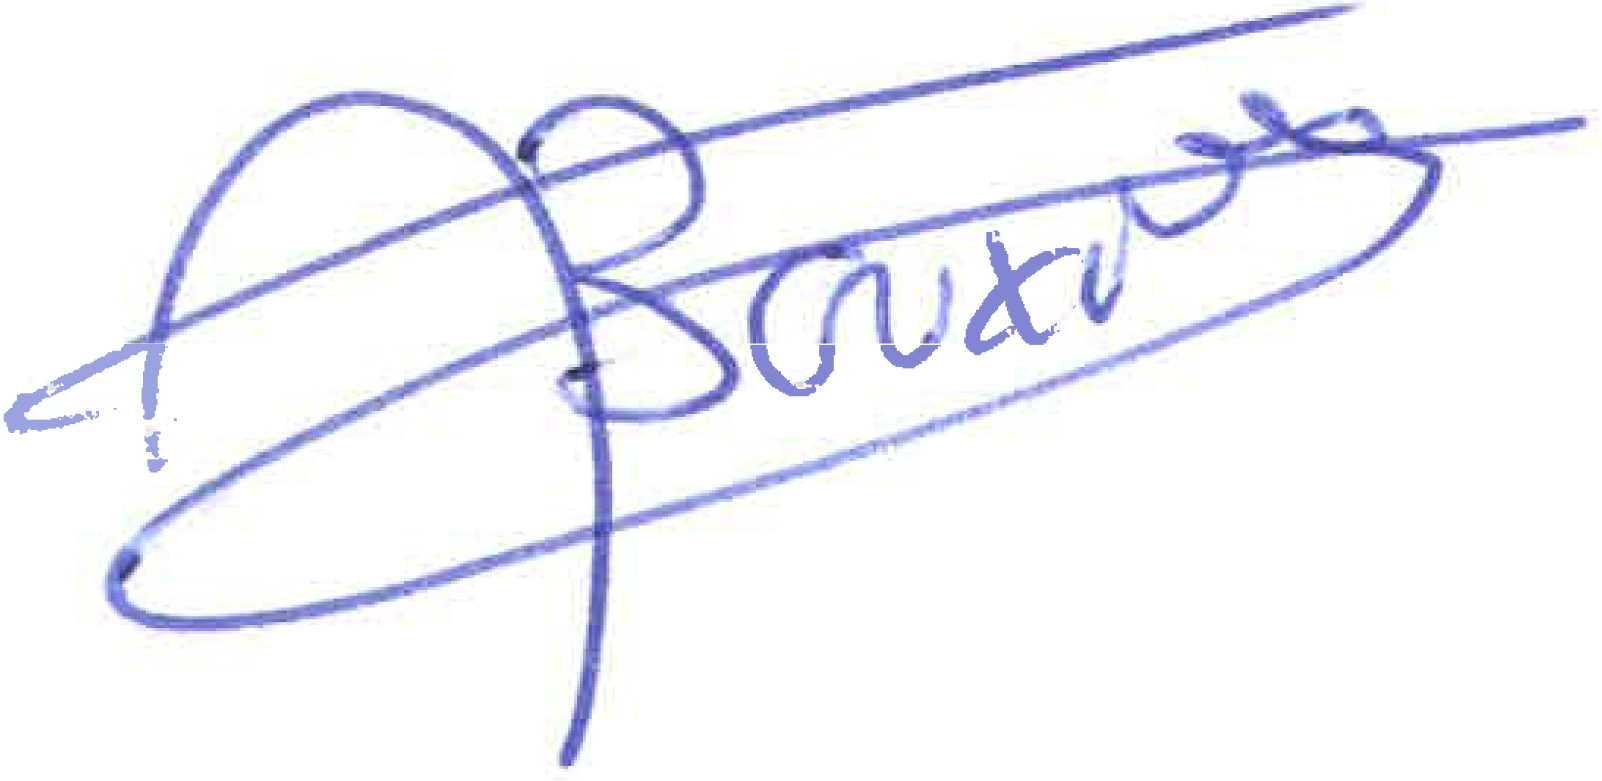
\includegraphics[width=\linewidth,height=15mm]{def/signatureAudreyBouxin.PNG}
\end{minipage} \\
Approved & L. Jolissaint & \today & \begin{minipage}{.2\textwidth}
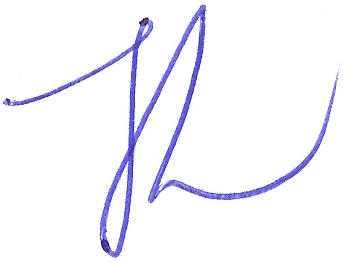
\includegraphics[width=\linewidth,height=15mm]{def/signatureLaurentAutographe.jpg}
\end{minipage} \\
& Name & October 10, 2017 & \dotfill \\
Released & Name & \today & \begin{minipage}{.2\textwidth}

\includegraphics[width=\linewidth,height=15mm]{def/signature.PNG}
\end{minipage} \\
& Name & \today & \dotfill \\
\end{tabular}
\end{center}

\lfoot{\vspace{5mm}
\includegraphics[width=\linewidth]{def/footpage.png}}

%\phantom{bla}
\newpage

%\hspace{-0.6cm}
\begin{center}
\begin{tabular}{llcl}
Issue & Date & Section/Page affected & Reason/Remarks \\ \hline
1.0 & October 10, 2017 & All & New \\ \hline
2.0 & May 18, 2018 & All & Review of all the design after decisions and Paolo Spano advices \\ \hline
\end{tabular}
\end{center}
\newpage

\setlength{\parindent}{0pt}%20pt}

%\tableofcontents

\section*{Acronyms}
\afterpage{\cfoot{\thepage}}

\begin{minipage}[c]{0.5\textwidth}
\begin{center}
\begin{tabular}{p{13mm}|p{55mm}}
aO & active Optics \\
AO & Adaptive Optics \\
CCD & Charge Coupled Device\\
CMOS & Complementary Metal Oxide Semiconductor\\
DAG & Dogu Anadolu Gozlemevi (East Anatolian Observatory)\\
DM & Deformable Mirror\\
FCL & Field Correction Lens\\
FoV & Field-of-View\\
FWHM & Full Width at Half Maximum\\
NCPA & Non Common Path Aberrations
\end{tabular}
\end{center}
\end{minipage}
\begin{minipage}[c]{0.5\textwidth}
\begin{center}
\begin{tabular}{p{16mm}|p{55mm}}
NGS & Natural Guide Star \\
OTF & Optical Transfer Function\\
P2V & Peak-to-Valley\\
PSF & Point Spread Function\\
PSF-R & PSF Reconstruction\\
PWFS & Pyramid WFS\\
RMS & Root Mean Square\\
SH-WFS & Shack-Hartmann WFS\\
SNR & Signal-to-Noise Ratio\\
TT & Tip-Tilt\\
WFS & Wavefront Sensor\\
WFE & Wavefront Error
\end{tabular}
\end{center}
\end{minipage}
\newpage

\section{Scope of this document}

This document presents the DAG adaptive optics (AO) optical train design and optimization.

\section{Introduction}
There are several mandatory points we have to handle :
\begin{itemize}
	\item the exit pupil has to be imaged on the DM (Deformable Mirror);
	\item the DM diameter is fixed to the DM-468 clear aperture from ALPAO; that means \O $33$ mm;
	\item the exit pupil of the telescope has to be imaged on the TT (Tip-Tilt) mirror for the P-WFS modulation;
	\item the beam has to converge on the pyramid apex;
	\item the angle of the beam that arrives onto the pyramid apex is calculated in order to get a diffraction limited PSF size of 2 times the pyramid roof;
	\item the exit pupil has to be imaged onto the Nuvu EMCCD detector;
	\item the beam footprint diameter onto the detector has to be defined accordingly to the oversampling criterion (explained section~\ref{subsec:Pup2CCD}).\\
\end{itemize}

We use off axis parabolas (OAPs) for all our design to reduce the aberrations (compared to lenses).
We have added one more constraint on the design which is to have parallel beam arriving or leaving each off axis parabola in order to limit the spherical aberrations.\\

The fixed parameters are resumed here :
\begin{itemize}
	\item exit pupil diameter : \diameter$_{\text{ExtP}} = 727.4046$ mm;
	\item distance exit pupil to focal plane : $\overline{\text{ExP-FP}} = 10338.74$ mm; 
	\item DM diameter : \diameter$_{\text{DM}} = 33.0$ mm;
	\item pixel size of the Nuvuu EMCCD AO : $\text{PxSize} = 24$ $\mu$m
\end{itemize}
\newpage
In order to design the AO bench we started with the telescope model. Indeed, we would try to compensate for the field of curvature introduced by the mirrors of the telescope with the off-axis parabolas (OAP) of the AO. The Zemax model of the telescope shows a curvature radius of about 1255 mm.
\begin{figure}[H]
	\begin{center}
		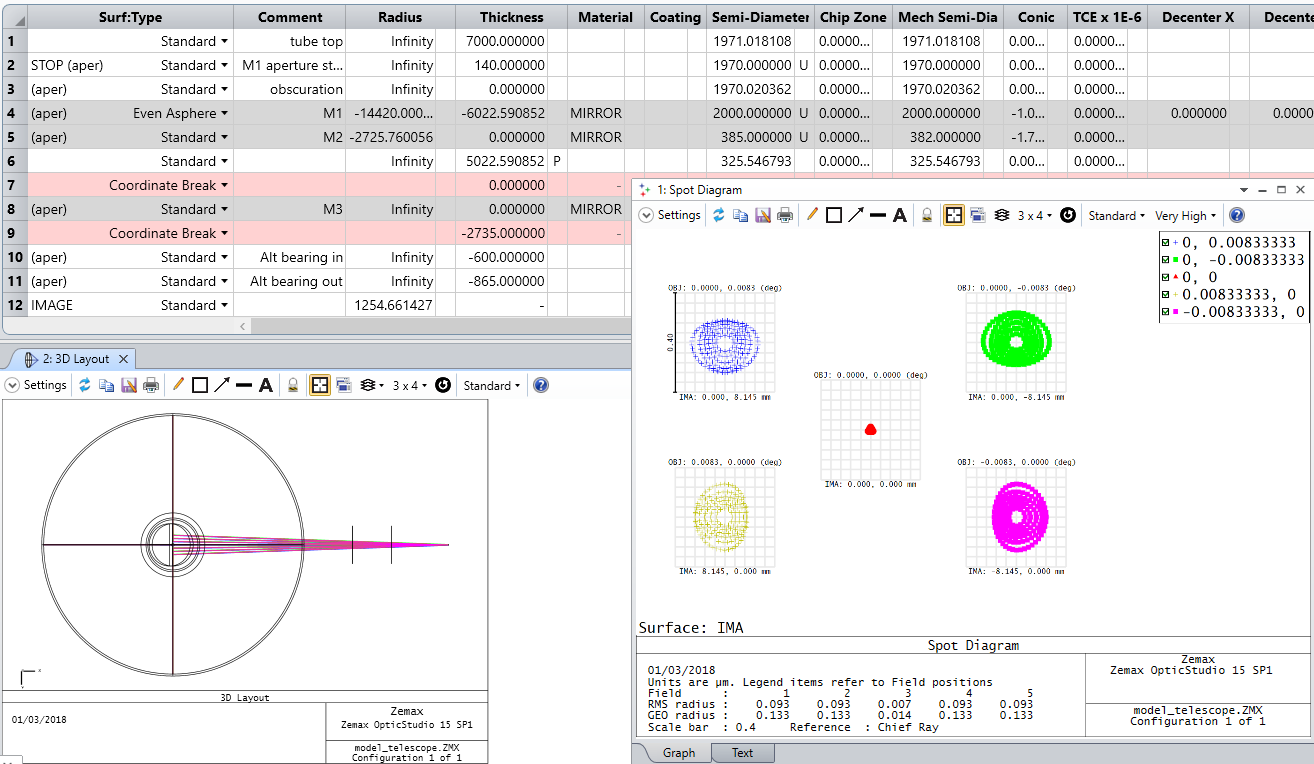
\includegraphics[width=\textwidth]{images/Zemax_model_telescope.PNG}
		\caption{Zemax model of the telescope}\label{fig:Zemax_model_telescope}
	\end{center}
\end{figure}

\newpage
\section{Design development and optimization}
A preliminary design have been set for the PDR and the main points are summarized at each optimization step of this report.

\subsection{Imaging the exit pupil of the telescope onto the DM}
The first branch consists on an imaging system of the telescope pupil onto the DM. The beam has to be collimated and the footprint has to take the entire clear aperture of the DM (for the DM-468 from ALPAO $\diameter_{\text{DM}}$~=~33~mm).\\
The beam on the DM has to be reflected with a certain angle otherwise the reflected beam comes back on itself. The maximum acceptable angle can be calculated considering the position error of the beam per actuator on the DM. We can align the beam with an error of $1/10^{th} \Lambda$ ($\Lambda$ the actuator pitch $= 1.5$ mm for the ALPAO DM-468). In order for the projected beam diameter to be no more than 10\% smaller than the DM diameter on both side, the tilt of the DM must be no more than $\alpha$~(figure \ref{fig:OAP0_DM_diam_beam_diam})~:
\begin{eqnarray}
	\alpha &= &\arccos\left(1-\frac{1}{5}\frac{\Lambda}{\diameter_{\text{DM}}}\right)\nonumber\\
	\alpha &= &\arccos\left(1-\frac{1}{5}\frac{1.5}{33}\right)\nonumber\\
	\alpha &= &7.73^{ \circ}\label{eq:alphaDM}\\
	2\alpha &= &15.46^{ \circ}\nonumber
\end{eqnarray}

\begin{figure}[H]
	\begin{center}
		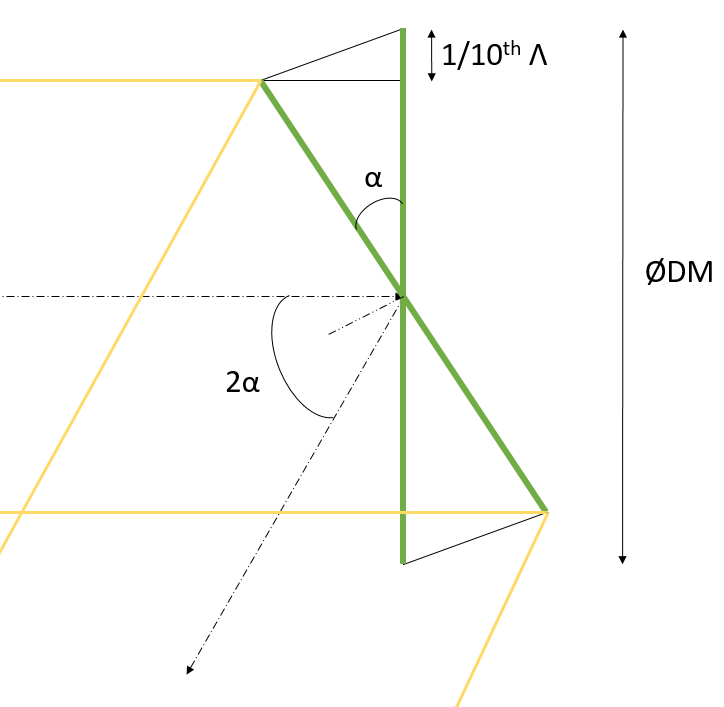
\includegraphics[width=0.3\textwidth]{images/OAP0_DM_diam_beam_diam.PNG}
		\caption{Sketch of the input and output beam depending on the tilt angle of the DM}\label{fig:OAP0_DM_diam_beam_diam}
	\end{center}
\end{figure}
The input beam diameter is then :
\begin{equation}
	\diameter_{\text{DM-beam}} = \diameter_{\text{DM}} \cos{\alpha} = 33\times \cos{(7.73)} = 32.7 \text{ mm}
\end{equation}

In order to have a collimated beam on the DM with a diameter of $\diameter_{\text{DM-beam}}$, the focal length of the OAP0 is calculated by the following sequence of equations. To visualize the parameters needed and the context we can look at figure~\ref{fig:sketch_ray_tracing_OAP0}. The with an angle $\theta$ with the corresponding reference coordinates $\left(0,x',y'\right)$. The ray $\Delta$CR corresponds to the chief ray, $\Delta\alpha u$ is the "upper" marginal ray and $\Delta\alpha b$ is the "bottom" marginal ray. The origin is placed at the focal plane of the telescope.

\begin{figure}[H]
	\begin{center}
		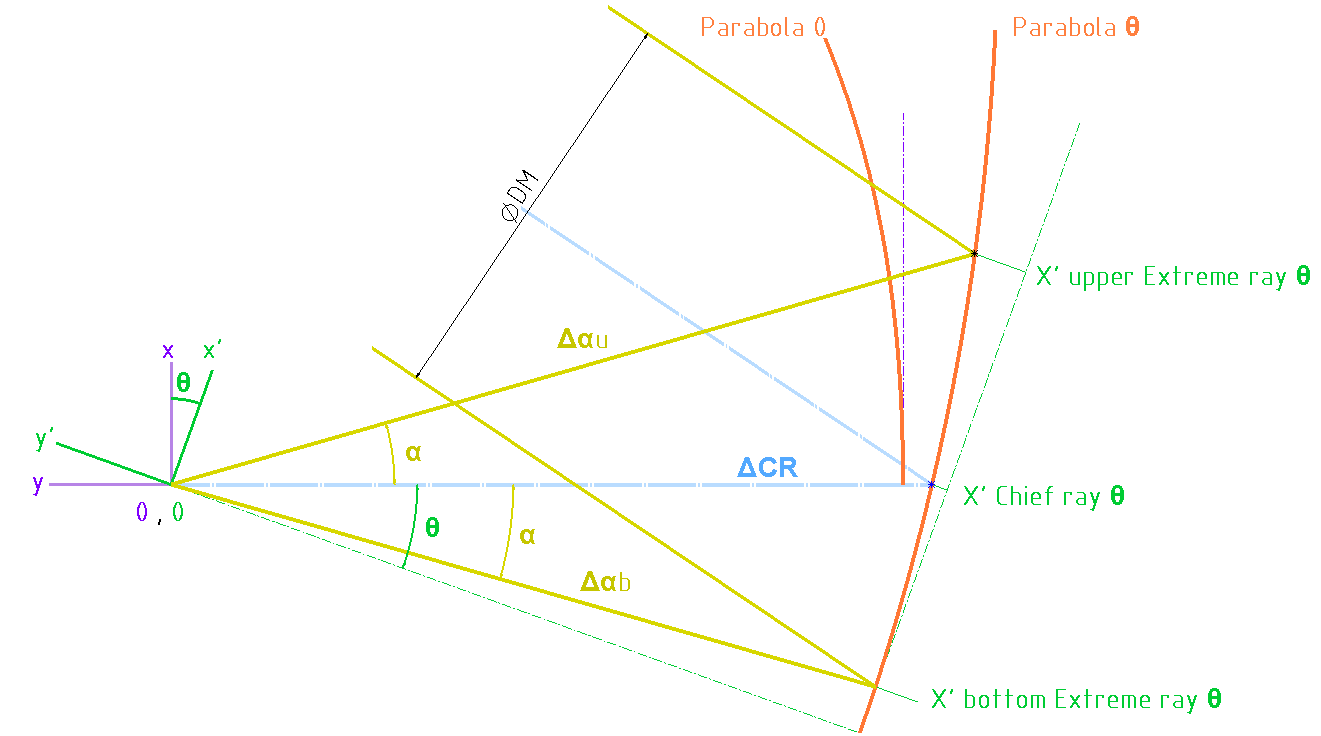
\includegraphics[width=.8\textwidth]{images/sketch_ray_tracing_OAP0.PNG}
		\caption{Ray tracing of a tilted parabola}\label{fig:sketch_ray_tracing_OAP0}
	\end{center}
\end{figure}
In the reference coordinates $\left(0,x',y'\right)$, we have (with PFL the Parental Focal Length of the OAP):
\begin{itemize}
	\item equation of the parabola $\theta$ : 
	\begin{equation}
	y' = \frac{x'^2}{4\,\text{PFL}}-\text{PFL}	\label{eq:parabola_theta}
	\end{equation}
	\item equation of $\Delta\alpha u$ : \begin{equation}
	y' = -\frac{1}{\tan\left(\theta+\alpha\right)}x' \label{eq:delta_alphau}
	\end{equation}
	\item equation of $\Delta\alpha b$ : \begin{equation}
	y' = -\frac{1}{\tan\left(\theta-\alpha\right)}x' \label{eq:delta_alphab}
	\end{equation}
\end{itemize}
%
%Determination of $x'_{\text{CR}\theta}$ (intersection between parabola $\theta$ and $\Delta$CR) :\\ \eqref{eq:parabola_theta} = \eqref{eq:delta_CR}\\
%\begin{equation}
%	x'_{\text{CR}\theta} = 2\,\text{PFL}\left(-\frac{1}{\tan\theta}+\sqrt{\frac{1}{\tan^2\theta}+1}\right)
%\end{equation}

Determination of $x'_{\text{Ex}\theta\,\,u}$ (intersection between parabola $\theta$ and $\Delta\alpha u$) :\\ \eqref{eq:parabola_theta} = \eqref{eq:delta_alphau}\\
\begin{equation}
	x'_{\text{Ex}\theta\,\,u} = 2\,\text{PFL}\left(-\frac{1}{\tan\left(\theta+\alpha\right)}+\sqrt{\frac{1}{\tan^2\left(\theta+\alpha\right)}+1}\right)
\end{equation}

Determination of $x'_{\text{Ex}\theta\,\,b}$ (intersection between parabola $\theta$ and $\Delta\alpha b$) :\\ \eqref{eq:parabola_theta} = \eqref{eq:delta_alphab}\\
\begin{equation}
	x'_{\text{Ex}\theta\,\,b} = 2\,\text{PFL}\left(-\frac{1}{\tan\left(\theta-\alpha\right)}+\sqrt{\frac{1}{\tan^2\left(\theta-\alpha\right)}+1}\right)
\end{equation}

In order to have the OAP0 output beam diameter equal to the DM clear aperture we have~:
\begin{equation}
	x'_{\text{Ex}\theta\,\,u}-x'_{\text{Ex}\theta\,\,b} = \diameter_\text{DM-beam}
\end{equation}
The parental focal length (see appendix~\ref{sec:EFL2PFL}) of OAP0 is :
\begin{equation}
	\text{PFL} = \frac{1}{2}\frac{\diameter_\text{DM-beam}}{-\frac{1}{\tan\left(\theta+\alpha\right)}+\sqrt{\frac{1}{\tan^2\left(\theta+\alpha\right)}+1}+\frac{1}{\tan\left(\theta-\alpha\right)}-\sqrt{\frac{1}{\tan^2\left(\theta-\alpha\right)}+1}}
\end{equation}
Using the equation~\eqref{eq:EFL2PFL} described in appendix~\ref{sec:EFL2PFL} we can transform the parental focal length into the effective focal length.\\

For the OAP0 the angle $\alpha_{\text{OAP0}}$ is
\begin{eqnarray}\label{eq:alpha_OAP0}
	\alpha_{\text{OAP0}} &= &\arctan\left(\frac{\diameter_{\text{ExP}/2}}{\overline{\text{ExP-FP}}}\right)
\end{eqnarray} 
The numerical application of \eqref{eq:alpha_OAP0} with $\diameter_{\text{ExP}} = 727.4046$ mm and $\overline{\text{ExP-FP}} = 10338.74$ mm gives $\alpha_{\text{OAP0}}  = 2.015\degree$, the aperture demi~angle of the beam arriving on the first OAP.\\

After the discussion we had with Paolo Spano, we took his advice into account and choose the parabola tilt angle according to the following precept : $\theta= 35\degree$ is a critical choice and $\theta > 35\degree$ is a nightmare (manufacturing and alignment). We should take an tilt angle smaller than 30$\degree$ to be realistic and the smaller the best. However, we are limited by the space around the focal plane because of the field correction lens (represented by the bloc on figure~\ref{fig:FCL_space_OAP0}). Depending on where it is going to be placed we would have to increase the angle of OAP0. \textbf{An email has been sent to AMOS who is going to design the FCL to know if it is possible to have it before the focal plane.}
\begin{figure}[H]
	\begin{center}
		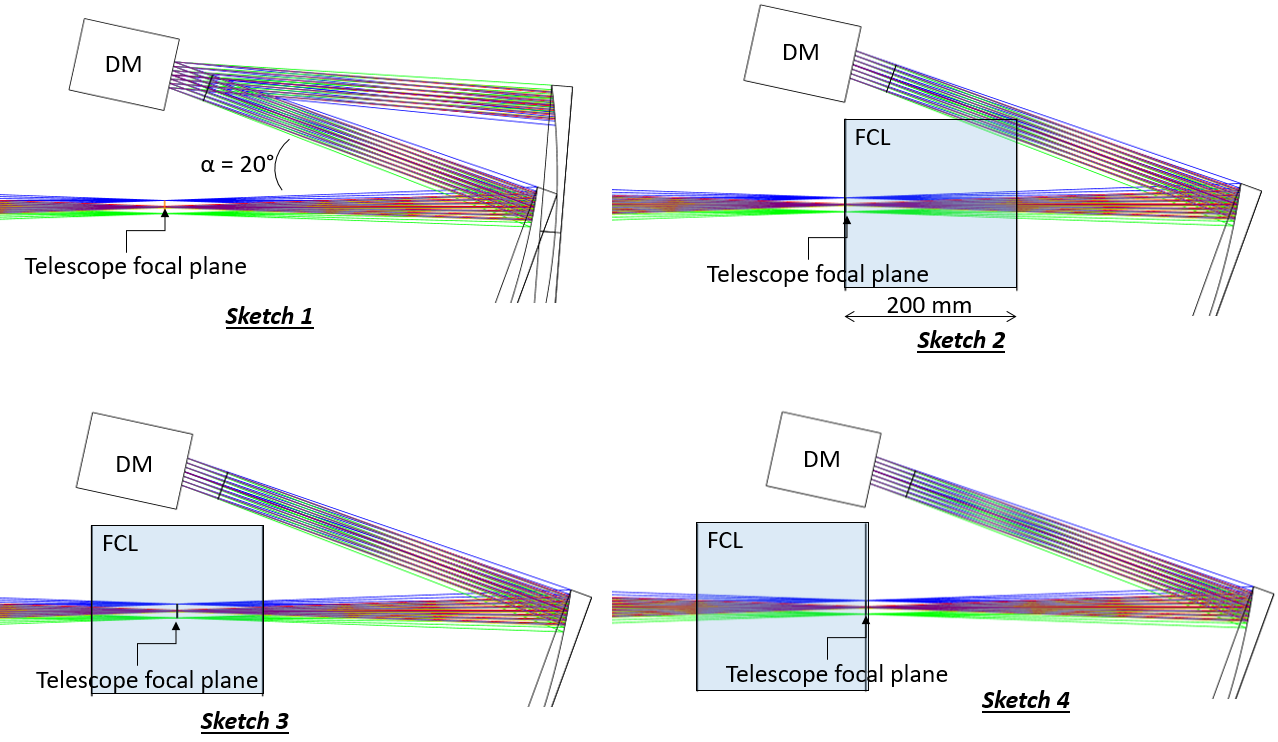
\includegraphics[width=.9\textwidth]{images/FCL_space_OAP0.PNG}
		\caption{Field correction lens position from the focal plane of the telescope}\label{fig:FCL_space_OAP0}
	\end{center}
\end{figure}

We  can set the parabola tilt angle to $\theta = 20\degree$ in order to keep this angle as small as possible to limit aberrations.\\

Using these inputs the focal length of the OAP0 is (appendix~\ref{app:DimensionnementOAPs}): $\text{PFL}_{\text{OAP0}} = 443.13\,\text{mm}	\nonumber$.\\
This value is too specific so we round it to\footnote{In Zemax, we enter the $\text{PFL}_{\text{OAP0}}$ and not the effective focal length in the coordinate break surface because using it, the translation is done before the tilt angle. This is why if we enter the translation in a surface before the coordinate break we cannot use the same length (we would then write the $\text{EFL}_{\text{OAP0}}$)}~:
\begin{equation}
	\text{PFL}_{\text{OAP0}} = 445\,\text{mm}	\nonumber
\end{equation}

\newpage
The image of the exit pupil given by OAP0 gives the position of the DM. Its position $p_i$ relative to the OAP0 vertex is given by (we use Gauss law)~:
\begin{eqnarray}
	p_i &= &\frac{p_o\,\text{PFL}_{\text{OAP0}}}{p_o+\text{PFL}_{\text{OAP0}}}\\
	p_i &= &\frac{-(10338.74+445)445}{-10338.74}\\
	p_i &= &464\,\text{mm}
\end{eqnarray}
The Zemax "pick up pupil position" macro is used to get the perfect DM position wrt the OAP0. The DM is then at $p_i = 493.08$ mm. Even if we understand that we cannot align the DM reflecting surface with this accuracy, we keep it in the Zemax model  and we will work on that during the tolerancing analysis\footnote{We always keep all the digit during an AO design in order to see what are the best results we can obtain with an ideal system.}. \\
The image of the pupil through a tilted OAP is also tilted~(see~\cite{cite:Design90degOAP}). This creates pupil aberrations.
\begin{figure}[H]
	\begin{center}
		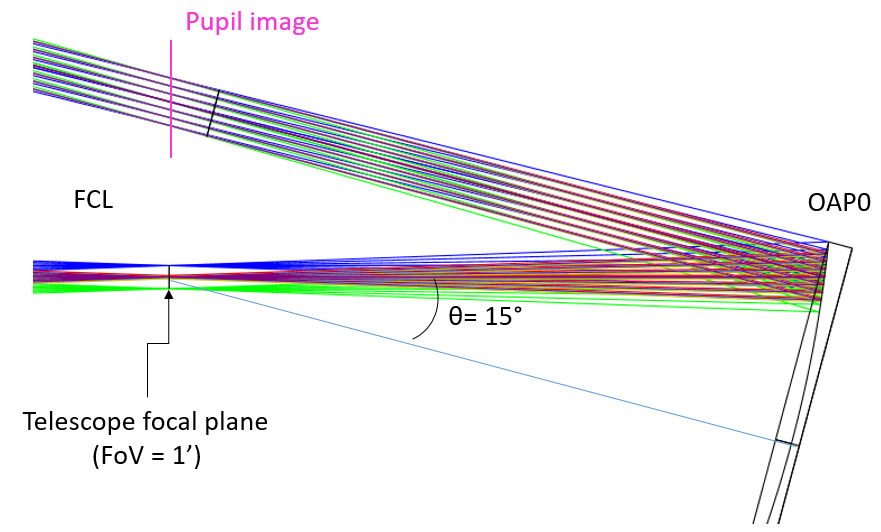
\includegraphics[width=.7\linewidth]{images/DM_pupil_tilt.PNG}
		\caption{Tilted image of the pupil}\label{fig:DM_pupil_tilt}
	\end{center}
\end{figure}
Here we want to place the DM at this pupil position. When we work with OAPs the image stop after an OAP is not perpendicular to the optical axis. The OAP introduce a tilt angle of the image plane. If we tilt the DM in the opposite position of this OAP-introduced tilt angle we add pupil aberrations whereas if we tilt it the same direction we can compensate for it. 

\begin{figure}[H]
%\centering
\begin{subfigure}[b]{0.45\textwidth}
	\begin{center}
		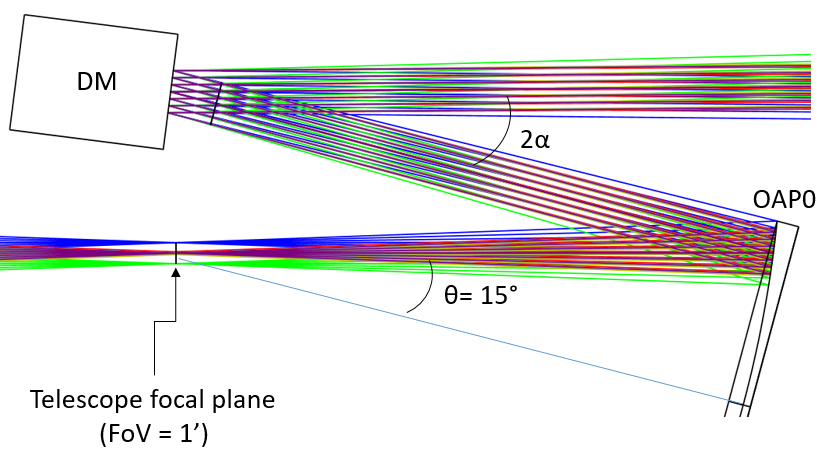
\includegraphics[width=\linewidth]{images/FP_OAP0.PNG}
		\caption{Layout}\label{fig:FP_OAP0}
	\end{center}
\end{subfigure}
\begin{subfigure}[b]{0.45\textwidth}
\begin{center}
		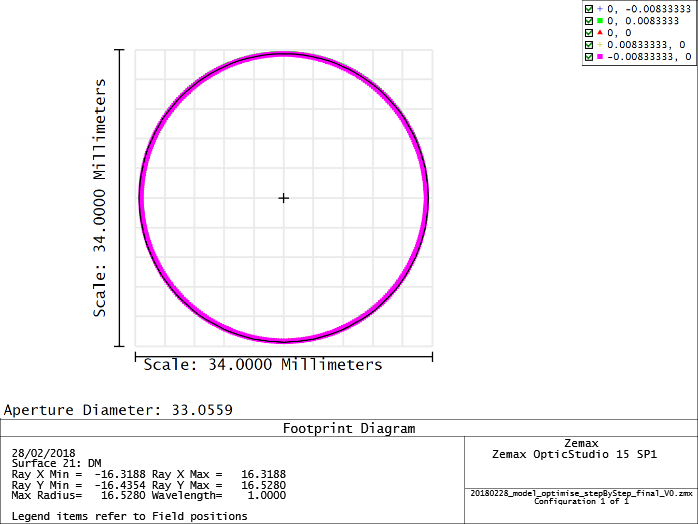
\includegraphics[width=\linewidth]{images/DM_beam_footprint.PNG}
		\caption{Zemax footprint diagram of the beam on the DM}\label{fig:DM_beam_footprint}
	\end{center}
\end{subfigure}
\caption{Zemax model of the 1rst part of the AO design}
\end{figure}

The beam footprint on the DM shows that all the field fits inside the clear aperture. The maximum diameter is equal to 32.7306 mm ($< 33$ mm). The angle of the DM is set to~-7.73\degree~(equation~\eqref{eq:alphaDM}),and not 7.73\degree as explain above.

\subsection{Imaging the pupil on the TT modulation mirror}

\subsubsection{Create an image of the pupil}
We need to image the pupil on the TT modulation mirror. Moreover, we know that to compensate for the introduced aberration from OAP0 we can use an OAP1 with the same focal length. The F/D ratio would stay the same as the telescope one which is favourable for the science path.\\
Figure~\ref{fig:Zemax_model_FP_OAP1} shows that to model this combination we use the "chief ray" solve on Zemax (Lens data) to keep the coordinates following the beam path (using the on-axis ray). OAP1 is placed at the exact inverse position of OAP0 in order to compensate for its aberrations so the intermediate focal plane is near the telescope focal plane.\\

\begin{figure}[H]
	\begin{center}
		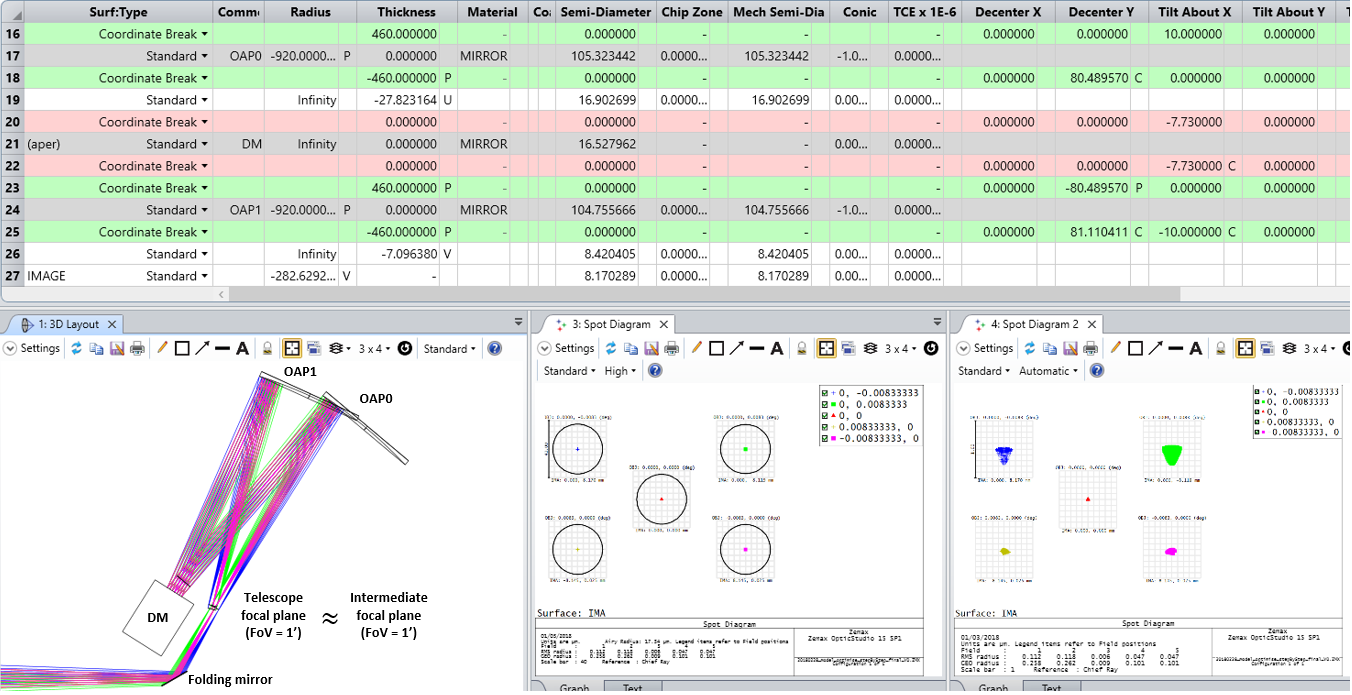
\includegraphics[width=\textwidth]{images/Zemax_model_FP_OAP1.PNG}
		\caption{Zemax model from the telescope beam to the intermediate focal plane}\label{fig:Zemax_model_FP_OAP1}
	\end{center}
\end{figure}
We use an optimization (smallest spot radius) to go to the best focal plane (surface \# 76 thickness is set as variable) and in order to consider the field curvature we set the radius of the image plane variable. The optimization using a merit function (Type~:~P2V, Criteria~:~Spot~Radius, Reference~:~Chief~Ray) is done on the image surface to get the smallest spot radius of the central beam (FoV = 0'). We can see that the spot diameter varies between 0.511~$\mu$m and 0.009~$\mu$m (the center of the FoV) but when we look the spots with the Airy disk we can say that the beam is well focused.\\
However, the radius of the image curvature is smaller than the telescope output field of curvature so we did not compensate for that, instead we increase it (we will see how we could work on that or not).\\

\subsubsection{Bend the beam}
We do not want the beam to go back in the field correction lens and we would like to place the dichroic nearby the intermediate focal plane. In order to do that properly, we fold the beam after the DM with a flat mirror.
\begin{figure}[H]
	\begin{center}
		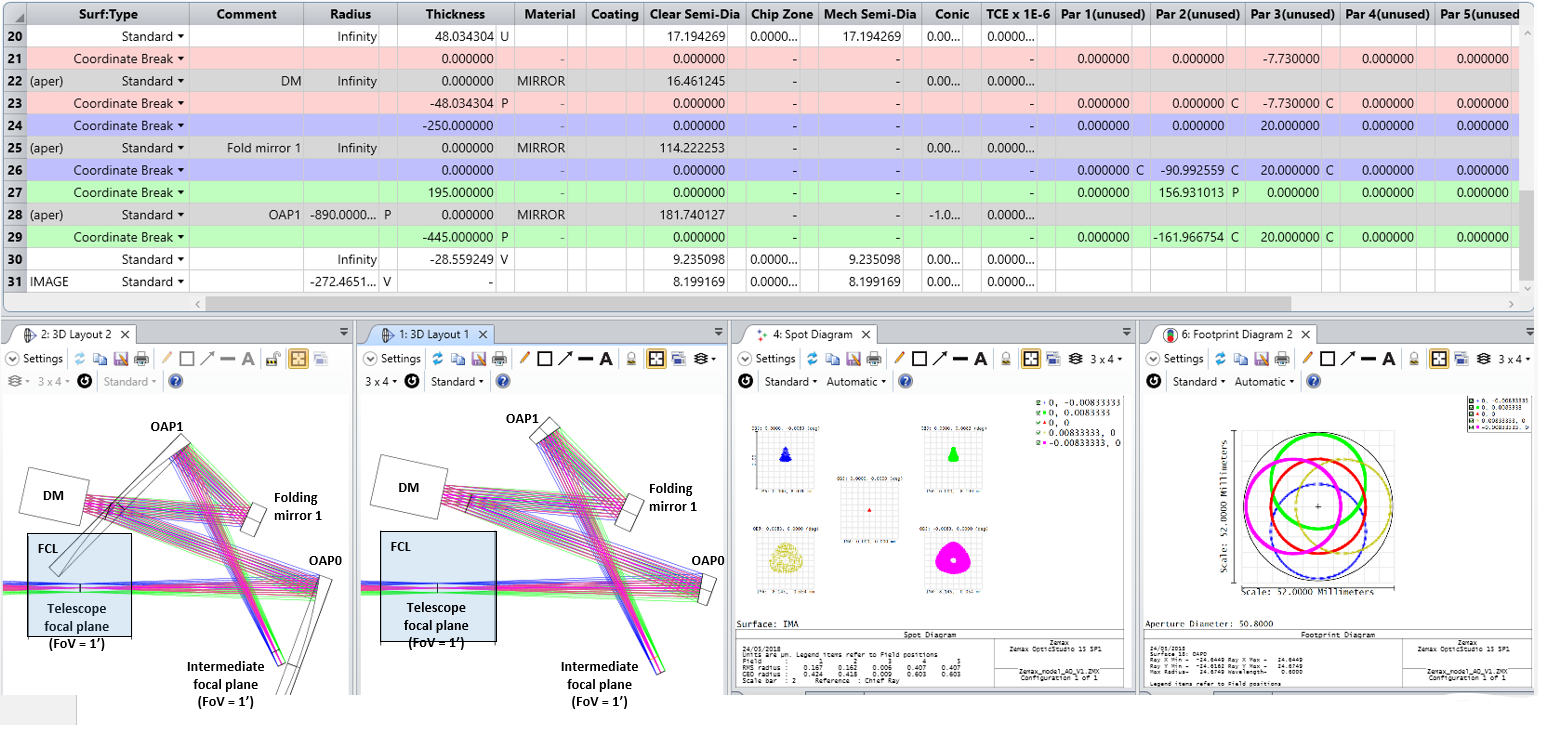
\includegraphics[width=\textwidth]{images/FP_2_intFP_FoldMirror.PNG}
		\caption{Zemax model from the telescope beam to the intermediate focal plane with a fold mirror after the DM}\label{fig:FP_2_intFP_FoldMirror}
	\end{center}
\end{figure}
Figure~\ref{fig:FP_2_intFP_FoldMirror} shows the new design with a folding mirror tilted at 20\degree. For more clarity we apply the real aperture size of the OAPs on layout 1. We can see on the footprint diagram that we can use two OAPs of 2~inches of diameter. The maximum diameter of the beam footprint (for a FoV~=~1') is about 49.9~mm. However, we should be careful and verify during the tolerance analysis that when we move the OAP in the alignment precision range we can do, the entire beam stays reflected on the OAP (no vignetting). Concerning the folding mirror, we can also use a diameter of 2~inches it is positioned at 298~mm from the DM (same as above, we have to check during the tolerancing that we do not have vignetting when moving around this position).\\

After redoing the optimization of the intermediate focal plane position and the image radius of curvature we found spot diameters vary from 0.009~$\mu$m (on-axis) to 0.603~$\mu$m (0.5') across the FoV (see figure~\ref{fig:IntermediateFP_SpotDiagram}).\\
\begin{figure}[H]
	\begin{center}
		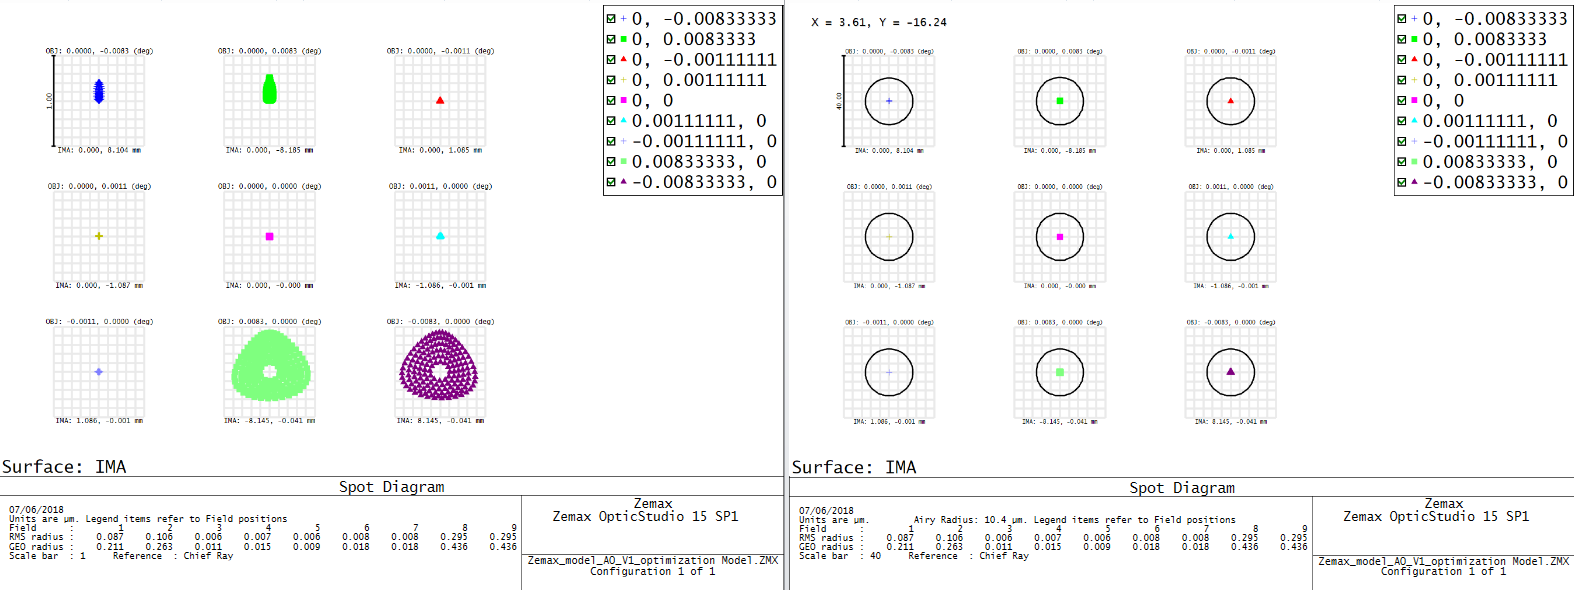
\includegraphics[width=.8\textwidth]{images/IntermediateFP_SpotDiagram.PNG}
		\caption{Spot diagram at the intermediate focal plane for the AO FoV and the WFS path FoV}\label{fig:IntermediateFP_SpotDiagram}
	\end{center}
\end{figure}

\subsubsection{Imaging the pupil on the TT modulation mirror}\label{subsubsec:TTMM}
\hl{The selection of the star in the FoV is made using an XY stage where all the WFS path would be mounted (as we have a compact WFS path).}
Now, as the OAP0 and OAP1 are the same, this optical configuration creates an image of the pupil of the same diameter at the same distance from the FP as the entrance pupil.\\ 
It is so not possible to use it to place the TT modulation mirror which has to be about 10~mm in diameter and at a reasonable distance from FP.
\hl{FOR these reasons........................................ we take a TT modulation mirror of \diameter 0.5~inch mounted on the fast tip-tilt platform S-331 from PI.}
We want to have a beam of about 10~mm in diameter at the pupil to place the TT stage.\\

We have also to note that we would like to introduce a dichroic membrane nearby the intermediate focal plane.

We know that we need to arrive on the pyramid roof (P-WFS) with a corresponding~:
\begin{equation}
	 F\#=2\frac{\text{pyramid roof}}{\lambda}\label{eq:FnumEq}
\end{equation}
Taking a pyramid roof of about $20~\mu$m according to Jean-Pierre Veran (private communication) at $\lambda~=~0.6~\mu$m we have~:
\begin{equation}
	F\# = 66.7\label{eq:Fnum}
\end{equation}
We round this value to F\#~=~60 (we need to investigate the pyramid roof size that can be manufactured).\\

We want then a vergence that takes the beam with a F\# of 14 and brings it to 60. The TT modulation mirror is placed in this converging beam at the pupil position. At first approximation, we can do a geometrical dimensioning. We use a drawing software and apply the constraints to calculate which focal length and distance from the intermediate focal plane we need. In order to build this ray tracing properly we calculate the following parameters~:
\begin{eqnarray}
	F\#_\text{input} = \frac{\overline{\text{ExP-FP}}}{\diameter_{\text{ExtP}}}\nonumber\\
	F\#_\text{output} = \frac{f_\text{lens}}{\diameter_\text{beam on the lens}}\nonumber\\
	\gamma_\text{input} = \frac{1}{2F\#_\text{input}}\nonumber\\
	\gamma_\text{output} = \frac{1}{2F\#_\text{output}}\nonumber
\end{eqnarray}
The image of the pupil is nearby the foci (at 0.06~mm) and has to be about 5~mm in diameter. Taking the angles and the beam diameter on the TT modulation mirror we find the focal length of the lens and the distance from the intermediate focal plane described figure~\ref{fig:SW_trace_rayons_lens_TTMM}.
\begin{figure}[H]
	\begin{center}
		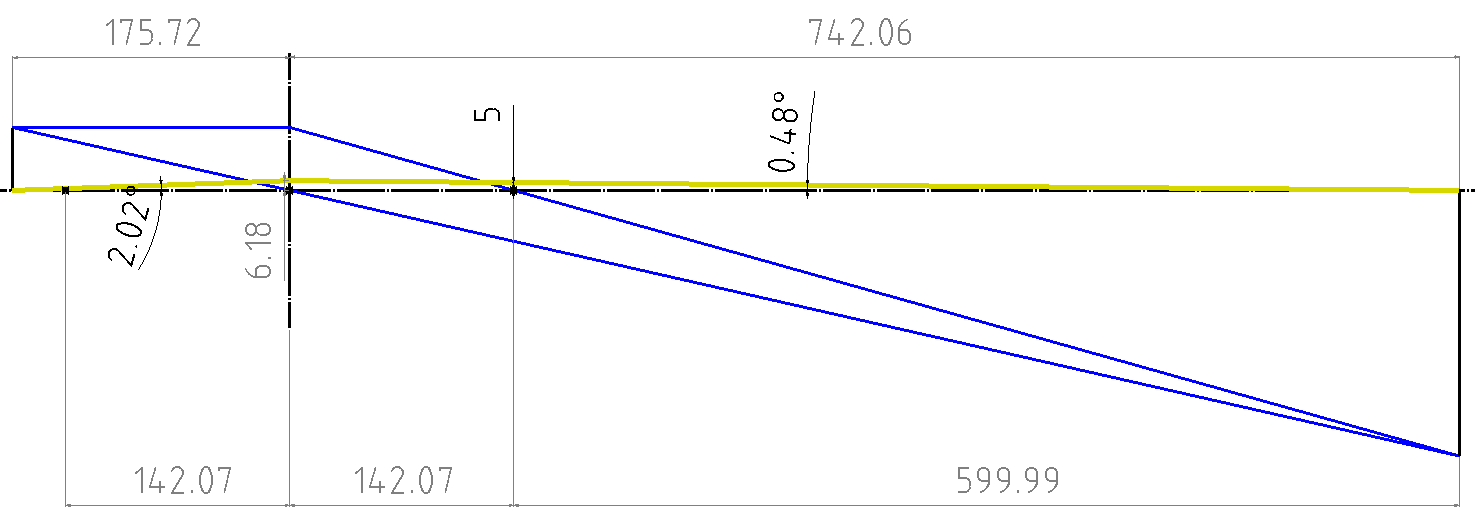
\includegraphics[width=.9\textwidth]{images/SW_trace_rayons_lens_TTMM.PNG}
		\caption{Ray tracing using SolidWorks to approximate the converging lens before the TT modulation mirror}\label{fig:SW_trace_rayons_lens_TTMM}
	\end{center}
\end{figure}
We introduce these results in Zemax using a paraxial lens (figure~\ref{fig:Zemax_model_FP_TTmod_noTilt}). We can see that the beam diameter is about 5~mm as expected.
\begin{figure}[H]
	\begin{center}
		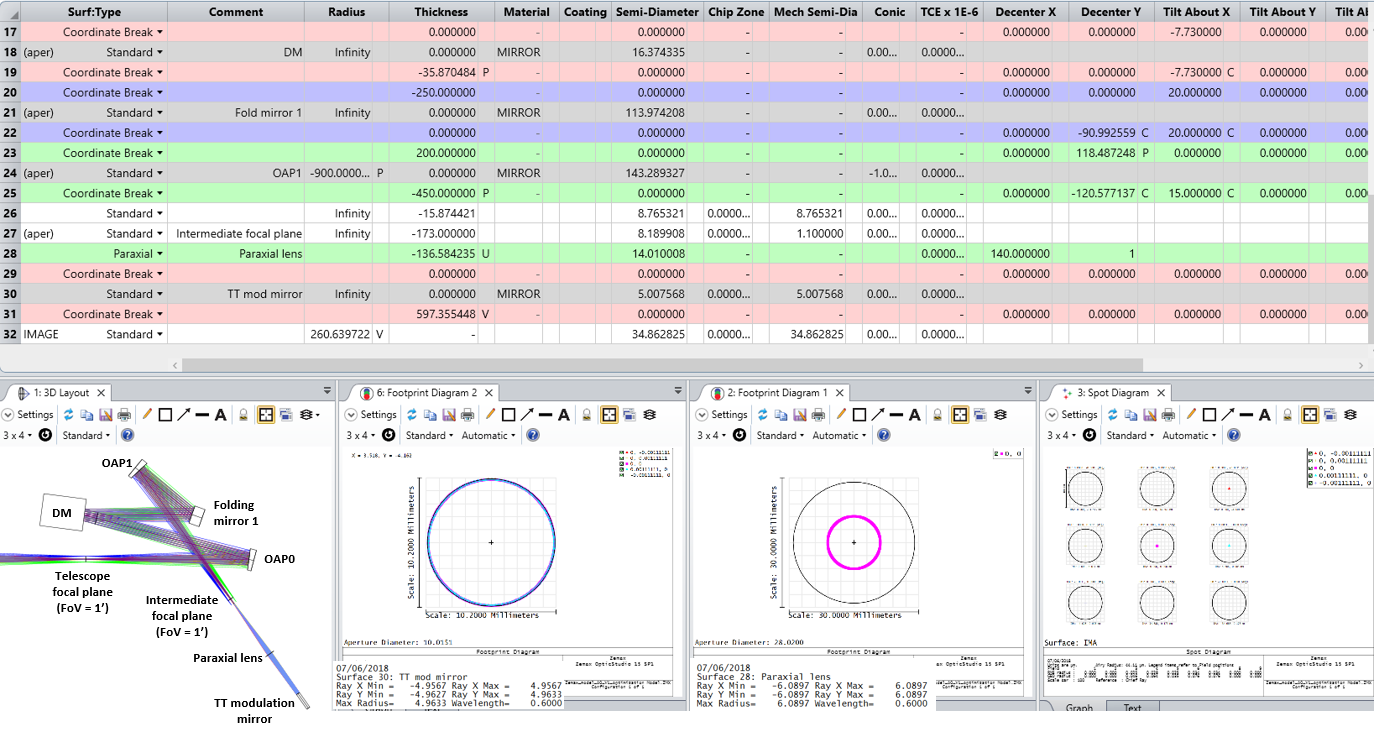
\includegraphics[width=\textwidth]{images/Zemax_model_FP_TTmod_noTilt.PNG}
		\caption{Zemax model from the telescope beam to the TT modulation mirror using a paraxial lens}\label{fig:Zemax_model_FP_TTmod_noTilt}
	\end{center}
\end{figure}
We want to tilt the TT modulation mirror to send the beam in a convenient direction. We need to add the ADC nearby a pupil plane, so if we want to use the pupil where the TT modulation mirror is placed we need some space around it to insert the ADC. We can tilt the TT modulation mirror with an angle of about 20\degree. The radius of the beam footprint on the TT modulation mirror measured on the Zemax model is~5.32~mm at maximum (which is smaller than 0.5~inch).\\
Moreover, the focal length of 142~mm is not a common value so we can change it to 140~mm.\\

We use the optimization tool to find the best focal plane (distance and radius of curvature at the image plane). As we are going to move all the WFS path with a XY stage to pick up the star, we can determine the beam footprint diameter on the paraxial lens with the on-axis case. We can see that the F\# of the beam arriving on the apex of the pyramid (figure~\ref{fig:Zemax_model_FP_TTmod_noTilt}) is F\#$~=~\frac{136.59+579.88}{7.1884*2}~=~58.5$ which is smaller than the F\#fixed before at 60. We can adjust it moving a little bit the paraxial lens from the intermediate focal plane. We find the final solution (figure~\ref{fig:Zemax_model_FP_ApexPyr}) with F\#$~=~\frac{136.59+597.35}{6.0897*2}~=~60.3$.\\
\begin{figure}[H]
	\begin{center}
		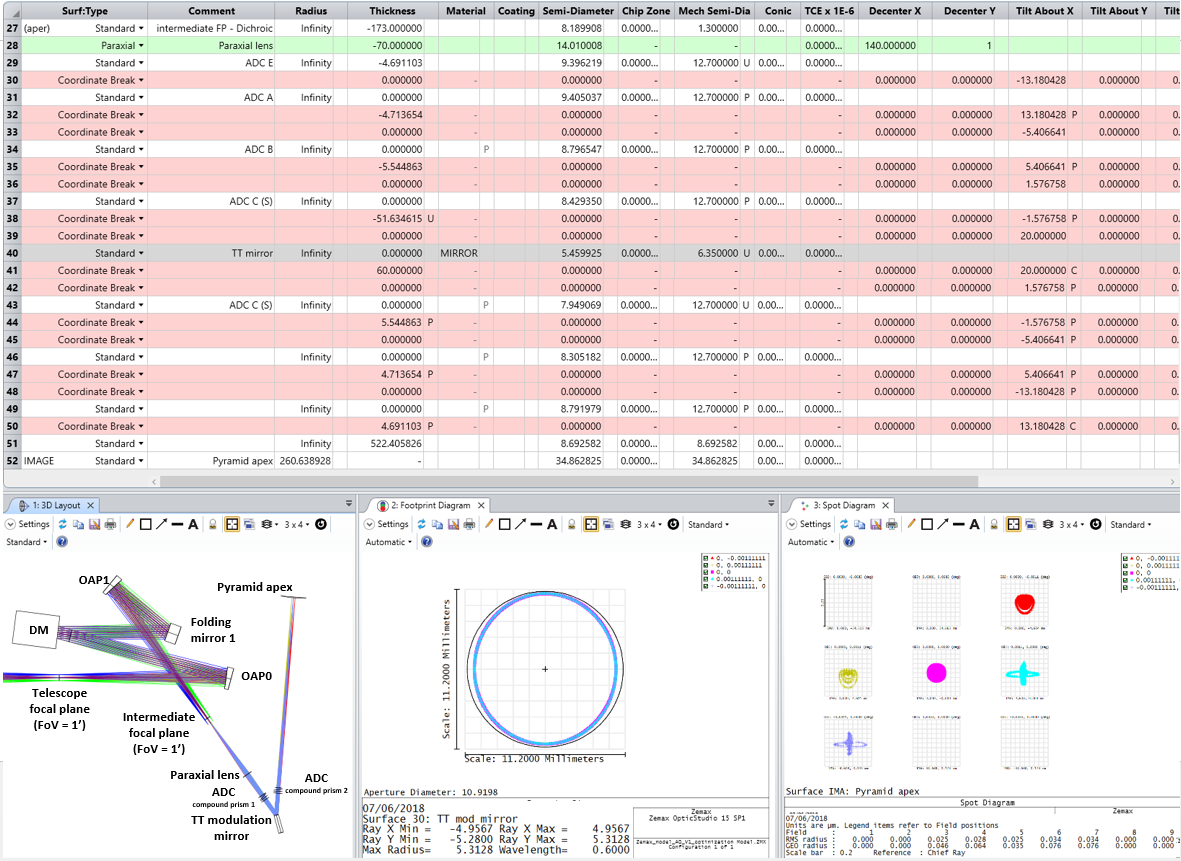
\includegraphics[width=\textwidth]{images/Zemax_model_FP_ApexPyr.PNG}
		\caption{Zemax model from the telescope beam to the apex of the pyramid WFS.}\label{fig:Zemax_model_FP_ApexPyr}
	\end{center}
\end{figure}

\hl{Actually, we could play with the angle of the TT modulation mirror to place the ADC closer to the pupil plane. This would be investigate according to the ADC design.}



\subsection{Image the pupil on the CCD detector}\label{subsec:4eme_partie}
The detector is the Nuvuu EMCCD with 128~pixels and a pixel size of $24~\mu$~m. We have to sample the beam with at least 1 pixel per actuator. In order to relax the alignment problems we can oversample the beam. According to Jean-Pierre Veran advice an oversampling of 1.5 should be enough. The ALAPO DM-468 has 22 actuators across the clear aperture diameter (so 23 pitches). Then we can calculate the beam diameter on the detector :
\begin{eqnarray}
	\diameter_{\text{CCD}} &= &\#_{\text{actuator across \diameter}}\times \text{PxSize}\times\text{Oversampling factor}\\
	\diameter_{\text{CCD}} &= &22\times 24~\mu\text{m}\times 1.5\\
	\diameter_{\text{CCD}} &= &0.792\,\,\text{mm}
\end{eqnarray}

The pupil has to be images on the camera through a relay lens. The pyramid does not act for the ray tracing and so the optical design, it separates the beam in four images only. We can look for the on-axis rays to dimension the relay lens and its position.\\
In order to play with the variables and have a direct result of what could be done or not, we used a sketch on the drawing software SolidWorks (figure~\ref{fig:SW_trace_rayons_TTMM_CCD}). Then, when you found something roughly fine we introduced the values in Zemax and optimized the distances in order to find the proper pupil plane and diameter.
\begin{figure}[H]
	\begin{center}
		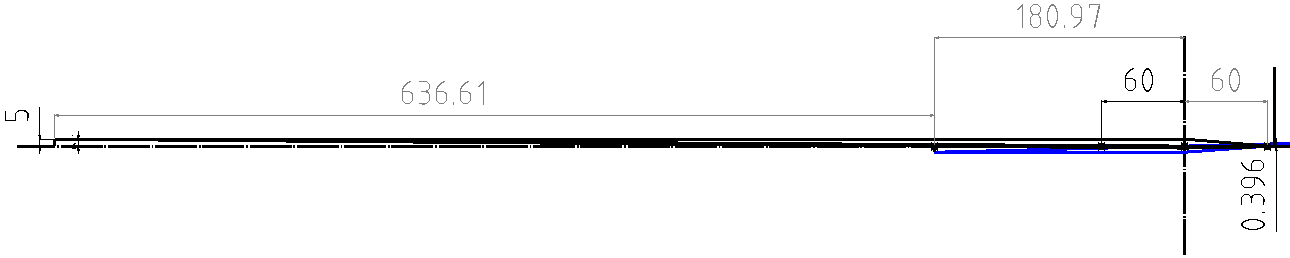
\includegraphics[width=\textwidth]{images/SW_trace_rayons_TTMM_CCD.PNG}
		\caption{SolidWorks ray tracing from the TT modulation mirror to the CCD.}\label{fig:SW_trace_rayons_TTMM_CCD}
	\end{center}
\end{figure}
We choose to fix the lens focal length in order to have a feasible lens. Playing with this distance we found that a lens of f~=~60~mm would be our best choice. The distance from the lens to the CCD detector is fixed by the pupil position solver in Zemax. The 
\begin{figure}[H]
	\begin{center}
		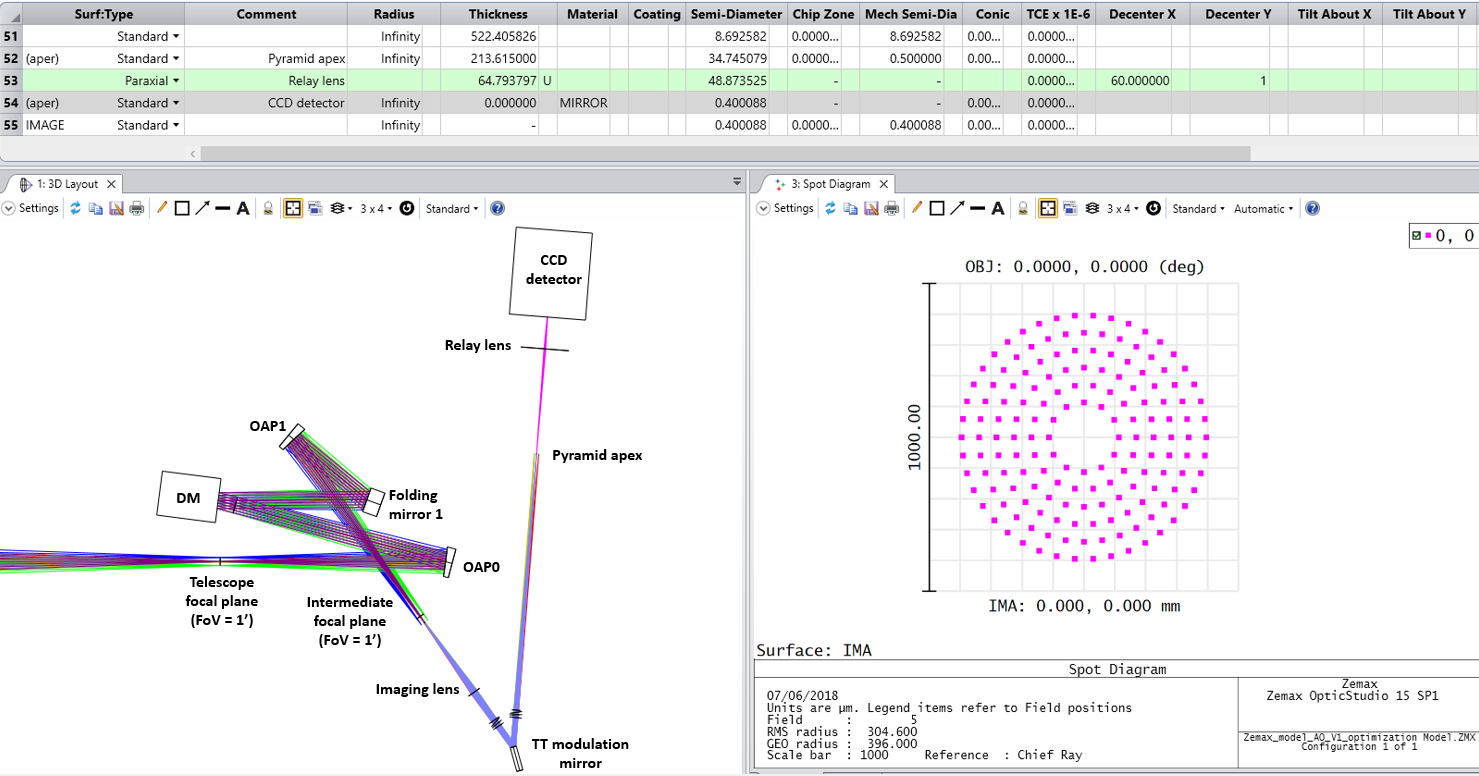
\includegraphics[width=\textwidth]{images/Zemax_model_FP_CCD.PNG}
		\caption{Zemax model of the bench until the CCD camera}\label{fig:Zemax_model_FP_CCD}
	\end{center}
\end{figure}
As said section~\ref{subsubsec:TTMM}, we would like to implement the WFS path on a XY stage to pick up the star in the FoV. The WFS path should be compact enough to place it on a platform not too large. This is the reason why we add a folding mirror before the pyramid apex. We can also think about adding a Z stage to the WFS path in order to realign the pupil when needed. This way we save space and we can consider the WFS path as a shoe box.
\begin{figure}[H]
	\begin{center}
		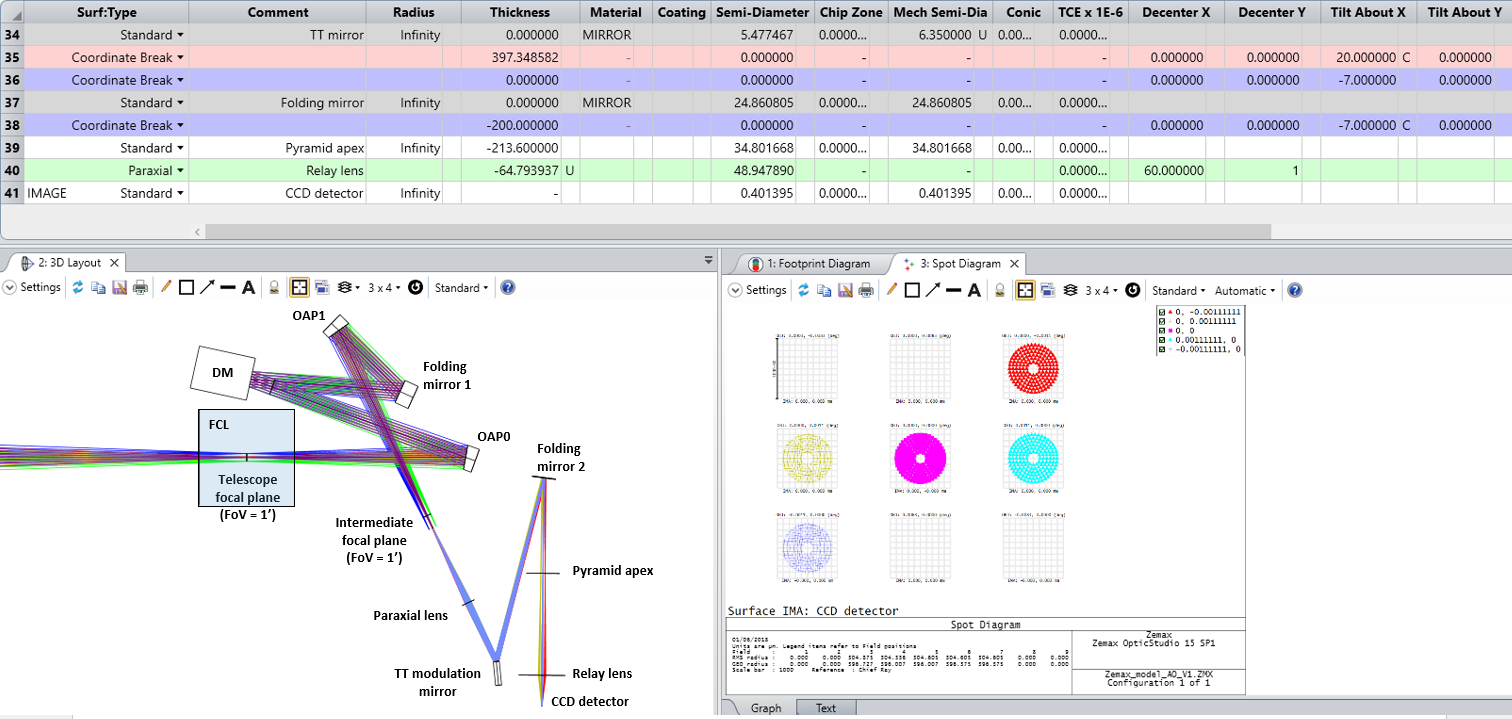
\includegraphics[width=\textwidth]{images/Zemax_model_FP_CCD_foldMirror.PNG}
		\caption{Zemax model of the bench until the CCD camera bending the beam}\label{fig:Zemax_model_FP_CCD_foldMirror}
	\end{center}
\end{figure}

\subsection{Atmopsheric Dispersion Compensator (ADC)}
We are designing an ADC to compensate the atmospheric dispersion (see appendix\ref{app:ADC}). The geometric parameters and the glass are not set yet this is why we do not have implemented it in the Zemax model for now. However, we can already say that the ADC would probably be inserted between OAP2 and OAP3 because the beam is collimated.
\newpage
% BIBLIOGRAPHIE
\bibliographystyle{ieeetr}
\renewcommand{\bibname}{References}
\bibliography{refbib/references_20180227_AO_design_report}
\addcontentsline {toc}{chapter}{References}
\addcontentsline {toc}{chapter}{Appendix}
\appendix
\newpage
\section{OAPs focal lengths relations}\label{sec:EFL2PFL}
This section describe the relation between the parental and the effective focal length for an off-axis parabola. The sketch figure~\ref{fig:EFL2PFL_sketch} describes the situation with :
\begin{itemize}
	\item EFL the effective focal length
	\item PFL the parental focal length
	\item ($x_S, y_S$) the coordinate of the ray intersection with the parabola
	\item the parabola of equation \begin{equation}
	y = \frac{x^2}{4\text{PFL}}-\text{PFL}	\label{eq:parabola_general}
\end{equation}	 
\end{itemize}

\begin{figure}[H]
	\begin{center}
		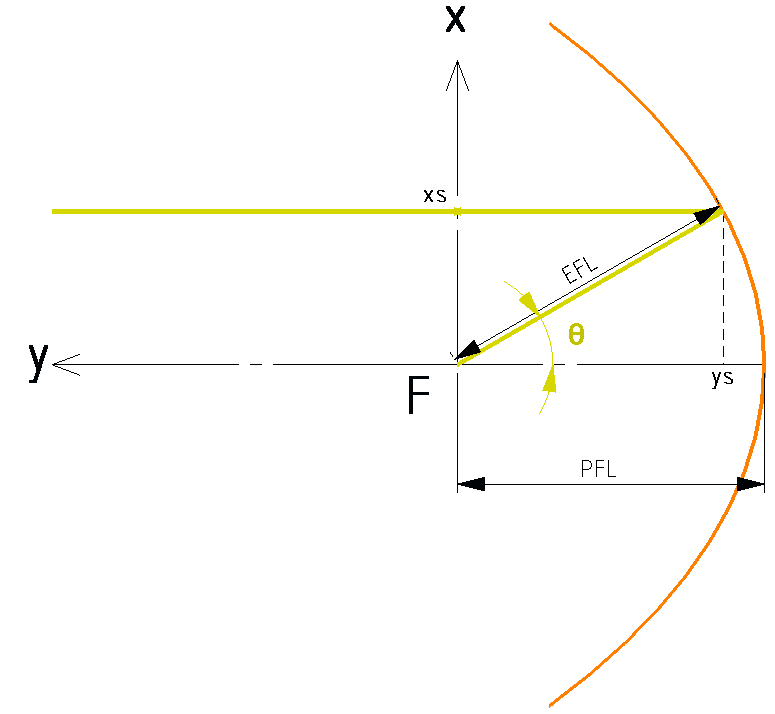
\includegraphics[width=0.5\textwidth]{images/EFL2PFL_sketch.PNG}
		\caption{Sketch of a ray reflected on an OAP}\label{fig:EFL2PFL_sketch}
	\end{center}
\end{figure}
The relation between EFL and PFL can be determined with the following set of equations.
\begin{eqnarray}
	x_S &= &\text{EFL}\sin\theta \nonumber\\
	y_S &= &\text{EFL}\cos\theta \label{eq:xs_ys}
\end{eqnarray}

Using \eqref{eq:parabola_general} and \eqref{eq:xs_ys} we have~:
\begin{eqnarray}
	4\text{PFL}\left(y_S+\text{PFL}\right) &= &x_S^2 \nonumber \\
	4\text{PFL}\left(\text{EFL}\cos\theta+\text{PFL}\right) &= &\left(\text{EFL}\sin\theta\right)^2\nonumber\\ 
	4\text{PFL}^2 - 4\text{PFL}\,\text{EFL}\cos\theta-\text{EFL}^2\sin^2\theta &= &0 \nonumber
\end{eqnarray}
\begin{eqnarray}
	\text{PFL}_{1,2} &= &\frac{4\text{EFL}\cos\theta\pm\sqrt{\left(-4\text{EFL}\cos\theta\right)^2+16\text{EFL}^2\sin^2\theta}}{2*4}  \nonumber\\
	&= &\frac{1}{2}\left[\text{EFL}\cos\theta\pm\sqrt{\text{EFL}^2\cos^2\theta+\text{EFL}^2\sin^2\theta}\right] \nonumber
\end{eqnarray}
The final equation is :
\begin{equation}
	2\text{PFL} = \text{EFL}\left(1+\cos\theta\right)\label{eq:EFL2PFL}
\end{equation}






%\newpage
%\section{Focal length of the relay lens between the pyramid and the CCD}\label{sec:PYR2CCD}
%Gauss :
%\begin{eqnarray}
%	\frac{1}{p_i}-\frac{1}{p_o} &= &\frac{1}{f_{LR}}	\nonumber\\
%	1-\frac{f_{LR}}{p_i} &= &-\frac{f_{LR}}{p_o}\label{eq:gaussPyr}
%\end{eqnarray}
%Thales :
%\begin{eqnarray}
%	\frac{\diameter_\text{CCD}}{\diameter_\text{L}} &= &\frac{|p_i|-|f_{LR}|}{|p_i|}\nonumber\\
%	\frac{\diameter_\text{CCD}}{\diameter_\text{L}} &= &1-\frac{f_{LR}}{p_i}\label{eq:ThalesPyr}
%\end{eqnarray}
%Mixing~\eqref{eq:gaussPyr} and \eqref{eq:ThalesPyr} :
%\begin{equation}
%	\frac{\diameter_\text{CCD}}{\diameter_\text{L}} = \frac{f_{LR}}{p_o}\label{eq:ThalGaussPyr}
%\end{equation}
%In another hand :
%\begin{equation}
%	\text{F}\# = \frac{f_\text{OAP3}}{\diameter_\text{TT}} = \frac{p_o}{\diameter_L}\label{eq:FnumPyr}
%\end{equation}
%Mixing \eqref{eq:ThalGaussPyr} and \eqref{eq:FnumPyr} :
%\begin{equation}
%f_\text{LR} = \text{F}\#\,\,\diameter_\text{CCD}
%\end{equation}



\newpage
\section{ADC design}\label{app:ADC}
\subsection{Scope}
The previous report explains the different possibilities to configure an ADC. Here we are presenting the design we are going to implement for the case of the DAG telescope AO. This ADC will be for visible wavelength. The range is limited by the camera Nuvu spectral range and the star spectrum studied. We are taking only the Nuvu camera bandwidth into account for a first iteration.\\

\subsection{Amici principle}
As said in the previous report, the Amici prisms are commonly used in the ADC systems. The ADCs are composed by a 2-doublet design which mixes two Amici prisms. This kind of prism is an alliance of two pieces of glass which have different dispersion (different refractive indexes). The materials must have the same refractive number for a mean wavelength so that at this frequency the incident and emergent rays are parallel (zero-deviation at $\lambda_{mean}$). The two prisms can be rotated around the optical axis in order to change the dispersion and compensate it for each wavelength. Shorter or longer wavelength than the middle one are deflected in opposite directions. When the angle between them is 180° the dispersion is reduced at its minimum.

\begin{figure}[H]
\centering
	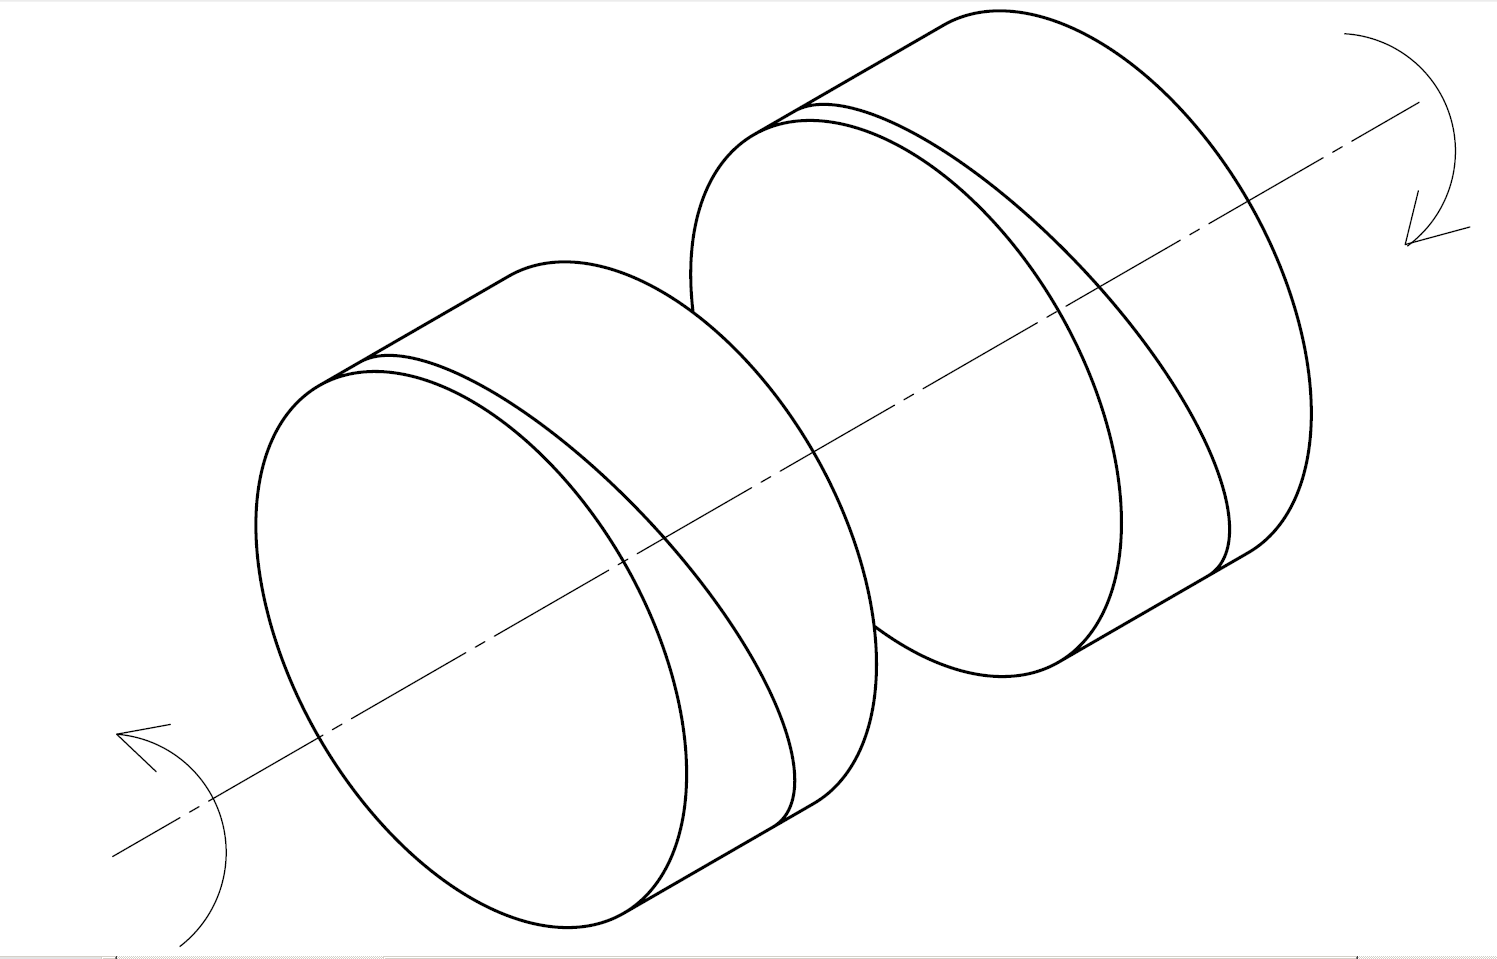
\includegraphics[width = 0.4\textwidth]{images/amiciISO.png}
	\caption{2-doublet Amici prisms design}
	\centering
\end{figure}



Another design can be a three-glass Amici prisms, which is called triplet-design. It consists of the insertion of a anomalous dispersion glass between the two firstly introduced surfaces.
\begin{figure}[H]
\centering
	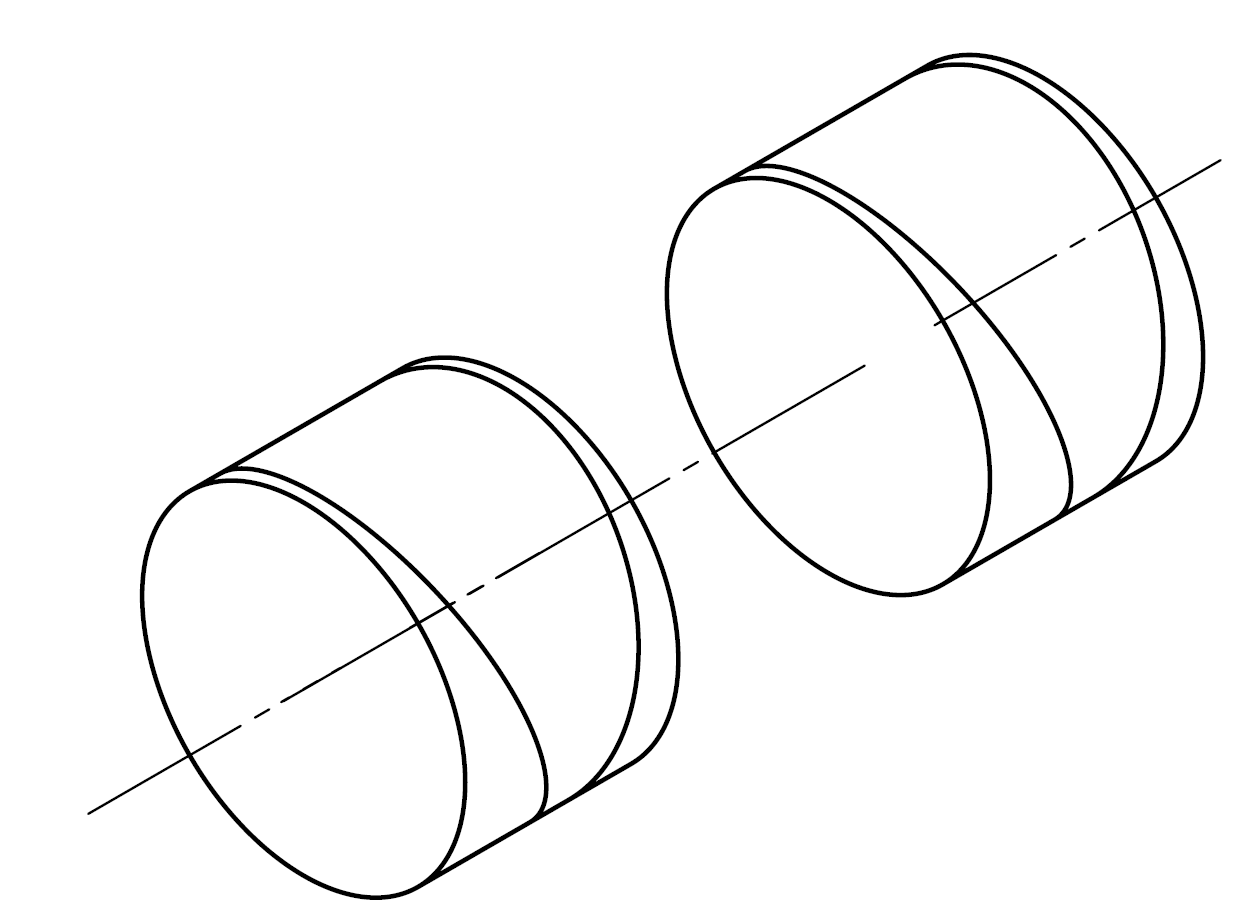
\includegraphics[width = 0.4\textwidth]{images/tripletDesignISO.png}
	\caption{2-triplet Amici prisms design \cite{KCG}}
	\centering
\end{figure}

The triplet-design seems to be appropriate for our case because it gives the best performance. According to Kopon thesis\cite{KCG}, the doublet corrects only the first order of chromatism while the triplet acts on both primary and secondary chromaticism aberration.\\

The system is made only by plane surfaces so that a plane front which go through the prisms should leave them as a plane front. In a collimated beam with a very narrow field of view the prisms combined thickness can be larger than the beam diameter \cite{Wynne1992}.\\
We can also use vertex with a certain radius in a converging beam. This way we can change the F\# leaving the ADC.\\
The doublet glass has to be designed in order to have a thermal expansion rate as close as possible between each glass to not break with the temperature changes. The internal reflection is also a parameter that we have to take into account because we want the ADC to transmit as much as possible light.\\

{ADC design}
In order to design our ADC, we need to collect some information about its position in the AO bench,the dispersion of the atmosphere for our parameters, the field of view (FoV) and wavelength bandwidth it has to work in.

\subsection{Model of the atmosphere refraction}

\subsubsection{Atmosphere refraction index}
First, we need to model to atsmophere dispersion (refractive index) depending on the wavelength. The simulation of the atmosphere refractive index is based on Ciddor's approach \cite{Ciddor} which is a compilation of all previous equations for the visible and near infrared. The following set of equations are used to model the atmosphere refraction :
\begin{eqnarray}
	10^8 \left(n_{as}-1\right) &= &k_1/\left(k_0-\sigma ^2\right)+k_3/\left(k_2-\sigma ^2\right)\\
	\left(n_{asx}-1\right) &= &\left(n_{as}-1\right) \left[1+0.534\times 10^{^-6}\left(x_c-450\right)\right] \label{eq:nasx}\\
		10^8 \left(n_{ws}-1\right) &= &1.022\times\left(\omega_0+\omega_1\sigma^2+\omega_2\sigma^4+\omega_3\sigma^6\right)\\
		n_{final} &= &\left(\rho_a / \rho_{axs}\right)\left(n_{axs}-1\right)+\left(\rho_\omega / \rho_{\omega s}\right)\left(n_{\omega s}-1\right)
\end{eqnarray}
where the parameters are defined as follow :
\begin{itemize}
	\item the wave number\\ $\sigma  = 2\pi/\lambda\,\,[\mu $m$^{^-1}]$
	\item Constants involved in the standard phase and group refractivities of dry air \cite{Ciddor}\\ $k_0 = 238.0185,\,k_1 = 5792105,\,k_2 = 57.362,\,k_3 = 167917\,\,[\mu $m$^{-2}]$ 
	\item $n_{as}$ the refractive index of standard air at T=20\degree C, 101325 Pa, 0 \% humidity, 450 ppm of CO$_2$
	\item for now, I took the concentration of CO$_2$ in the air of x$_c$ = 450 ppm (standard) so equation~\eqref{eq:nasx} becomes $n_{asx} = n_{as}$ but we can change that easily changing the x$_c$ parameter in the code
	\item $n_{asx}$ the refractive index of $x_c$ ppm of CO$_2$ at T=20\degree C, 101325 Pa, 0 \% humidity
	\item Constants involved in the standard phase and group refractivities of water vapor\cite{Ciddor}\\ $\omega_0 = 295.235\,[\mu $m$^{-2}],\,\,\omega_1 = 2.6422\,[\mu $m$^{-2}],\,\,\omega_2 = -0.032380\,[\mu $m$^{-4}],\,\,\omega_3 = 0.004028\,[\mu$m$^{-6}]$
	\item $n_{\omega s}$ the refractive index of water vapour at T=20\degree C, 1333 Pa
	\item $\rho_a$ [kg/m$^3$] the humid air density calculated equation~\eqref{subsubsec:rho_a}
	\item $\rho_{axs}$ [kg/m$^3$] the density of dry air at standard conditions calculated equation~\eqref{subsubsec:rho_axs}
	\item $\rho_\omega$ [kg/m$^3$] the density of water vapour calculated equation~\eqref{subsubsec:rho_w}
	\item $\rho_{\omega s}$ [kg/m$^3$] the density of water vapour at standard conditions calculated equation~\eqref{subsubsec:rho_ws}
\end{itemize}

\paragraph*{Calcul of the humid air density}
\begin{eqnarray}
	\rho_a &= & \frac{P\,M_a}{Z\,R\,T}\left[1-x_V\left(1-\frac{M_V}{M_a}\right)\right]\label{subsubsec:rho_a}\\
	P &= & P_0\left(1-\frac{\Delta T\,H}{T}\right)^{\frac{g\,M_a}{R\Delta T}}\nonumber\\
	M_a &= &\left(28.9635+12.011(xCO2-0.0004)\right)\times 10^{^-3}\nonumber\\
	Z &= &1-\frac{P}{T}\left[a_0+a_1\,t+a_2\,T^2+\left(b_0+b_1\,t\right)*x_v +(c_0+c_1\,t)*x_v^2\right] +\frac{p^2}{T^2}\left(d+e*xv^2\right)\nonumber
\end{eqnarray}
with :
\begin{itemize}
	\item $P_0 = 1.01325\times 10^5$ [Pa] the normal pressure at altitude 0 m;
	\item $P$ the pressure at altitude $H$ \cite{app:Wiki_HumidDensityAir};
	\item $g = 9.80665$ [m/s$^2$] earth-surface gravitational acceleration;
	\item $\Delta T = 0.0065$ [K] the vertical gradient of temperature (0.65K for 100 m)\cite{wiki_DP}
	\item $T_0 = 15$ [\degree C] sea level standard temperature
	\item $T = -10$ [\degree C] mean temperature from DAG-AWOS1
	\item $H = 3170$[m] Karakaya altitude
	\item $M_a$ [kg/mol] the density of dry air with $xCO2 = 0.0004$ \cite{Davis1992}
	\item $M_V = 18.01528\times 10^{-3}$ [kg/mol] the mole mass of water
	\item $R = 8.314510$ [J/mol/K] the molar gas constant
	\item $Z$ the compressibility with $t$ the temperature in [\degree C] and the following constants and parameters \cite{Davis1992} :\\
	\begin{itemize}
		\item $a0 = 1.58123\times 10^{-6}\,[$K*Pa$^{-1}],\,\,a1 = -2.9331\times 10^{-8}\,[$P$a^{-1}],\,\, a2 = 1.1043\times 10^{-10}\,[$(K*Pa)$^{-1}]$, $b0 = 5.707\times 10^{-6}\,[$K*Pa$^{-1}],\,\,b1 = -2.051\times 10^{-8}\,[$Pa$^{-1}],\,\,c0 = 1.9898\times 10^{-4}\,[$K*Pa$^{-1}]\,\,c1 = -2.376\times 10^{-6}\,[$Pa$^{-1}],\,\,d  = 1.83\times 10^{-11}\,[$K$^2$Pa$^{-2}],\,\,e  = -0.765\times 10^{-8}\,[$K$^2$Pa$^{-2}]$
		\item $x_v = $RH$\,f\frac{P_{sv}}{P}$ mole fraction of water vapour, RH the relative humidity (taken here as 0.8)
		\item $f = \alpha+\beta P+\gamma T^2$ increasing factor ($\alpha = 1.00062$ [-], $\beta  = 3.14\times 10^{-8}$ [Pa], $\gamma = 5.6\times 10^{-7}$ [K$^{-2}$])
		\item $Psv = \exp\left(AT^2+BT +C+\frac{D}{T}\right)$ the saturation vapour pressure of moist air ($A = 1.2378847\times 10^{-5}$ [K$^{-2}$], $B = -1.9121316\times 10^{-2}$ [K$^{-1}$], $C = 33.93711047$ [-], $D = -6.4341645\times 10^3$ [K])
	\end{itemize}	 
\end{itemize}

\paragraph*{Calcul of density of dry air at standard conditions (\cite{app:Wiki_HumidDensityAir}, \cite{airDensityBrisbane})}
\begin{equation}
	\rho_{axs} = \frac{P_0}{R_{gas}T_0}\label{subsubsec:rho_axs}
\end{equation}
with $R_{gas} = 287.05$ [J/kg/K] \cite{airDensityBrisbane}.

\paragraph*{Calcul of the water vapour density}
\begin{equation}
	\rho_\omega = \frac{P_wM_V}{R\,T}\label{subsubsec:rho_w}
\end{equation}
With :
\begin{itemize}
	\item $M_V = 18.01528\times 10^{-3}$ [kg/mol] the mole mass of water
	\item $P_w$ [mb] partial pressure of water vapour (mmHg2Pa = 133.322365 and $Psat$ [mmHg] valid between  -50\degree C and 200\degree C)
\end{itemize}

\begin{eqnarray}
	Psat &= &\exp\left(46.784-\frac{6435}{T}-3.868\log(T)\right)\nonumber\\
	Pw &= &Psat*RH*\text{mmHg2Pa}\nonumber
\end{eqnarray}	

\paragraph*{Calcul of the water vapour density at standard conditions}
\begin{equation}
	\rho_{\omega s} = \frac{P_{w0}M_V}{R\,T_0}\label{subsubsec:rho_ws}
\end{equation}
With :
\begin{itemize}
	\item $M_V = 18.01528\times 10^{-3}$ [kg/mol] the mole mass of water
	\item $P_{w0}$ [mb] partial pressure of water vapour (mmHg2Pa = 133.322365 and $Psat0$ [mmHg] valid between  -50\degree C and 200\degree C)
\end{itemize}

\begin{eqnarray}
	Psat0 &= &\exp\left(46.784-6435/(T0)-3.868\log(T0)\right)\nonumber\\
	P_{w0} &= &Psat0*RH*\text{mmHg2Pa}\nonumber
\end{eqnarray}	


\subsubsection{Atmosphere refraction equation}
The refraction of the atmosphere is computed with the equation \cite{Stone1996}: 
\begin{equation}
	R(\lambda,z) = \kappa\left(n(\lambda)-1\right)\left(1-\beta\right)\tan(z) - \kappa\left(n(\lambda)-1\right)\left(\beta -\frac{\left(n(\lambda)-1\right)}{2}\right)\tan^3(z)\label{eq:Ratm}
\end{equation}
with 
\begin{itemize}
	\item $\beta = 0.001254\left(\frac{T(K)}{273.15}\right)$ the effective height of the observatory above the surface of the earth \cite{Stone1996}
	\item $\kappa = 1$ for a spherical Earth surface \cite{Stone1996} or instrumental correction no more useful \cite{Stone2002}
\end{itemize} 
This equation~\eqref{eq:Ratm} is valid only for zenith angle < 75\degree. We can even neglect the second term for zenith angles < 65\degree \cite{Tendulkar}. The limit of zenith angle of our computation is set to 70\degree so the entire equation is set.









\subsubsection{Glasses for the ADC}
The choice of glass depends on the range of zenith angles, the wavelength interval, the maximum size of the blanks and the cost \cite{WynneWors1986}). Most of the glass couple in the Amici conception are flint/crown pairs plus an anomalous dispersion glass inserted for the triplet design. \\
The glass choice is made in a data base built from Schott and Ohara catalogues. The data are taken from~\cite{RefIndexInfo} where we can download glasses properties from many different suppliers. The data are sorted to extract Sellmeier coefficients~\cite{SchottSellmeier} in order to compute the refractive index of each glass depending on the wavelength with the equation~\eqref{eq:Sellmeier}.

\begin{equation}
	n^2(\lambda) = 1+ \frac{B_1\lambda^2}{\lambda^2-C_1}+\frac{B_2\lambda^2}{\lambda^2-C_2}+\frac{B_3\lambda^2}{\lambda^2-C_3}\label{eq:Sellmeier}
\end{equation}
with $B_i$ and $C_i$ Sellmeier coefficients for $\lambda$ in $\mu$m~\cite{SchottSellmeier}.\\

The final glass data base with the refractive index reported is generated for three wavelengths : le smallest, the highest and the mean wavelength. These are for our case the Nuvu camera~\cite{NuvuQE} bandwidth limits $\lambda_{min} = 0.3\,[\mu m]$ and $\lambda_{max} = 1.0\,[\mu m]$ and the maximum quantum efficiency corresponding wavelength $\lambda_{mean} = 0.6\,[\mu m]$.














\subsubsection{Beam propagation through the ADC}
In order to compute de dispersion through the ADC a geometrical and refraction set of equations have been implemented. The sequence of these equations is listed bellow. I will follow the light on the figure~\ref{fig:ADCgeometrie} to describe each step.
\begin{figure}[H]
\centering
	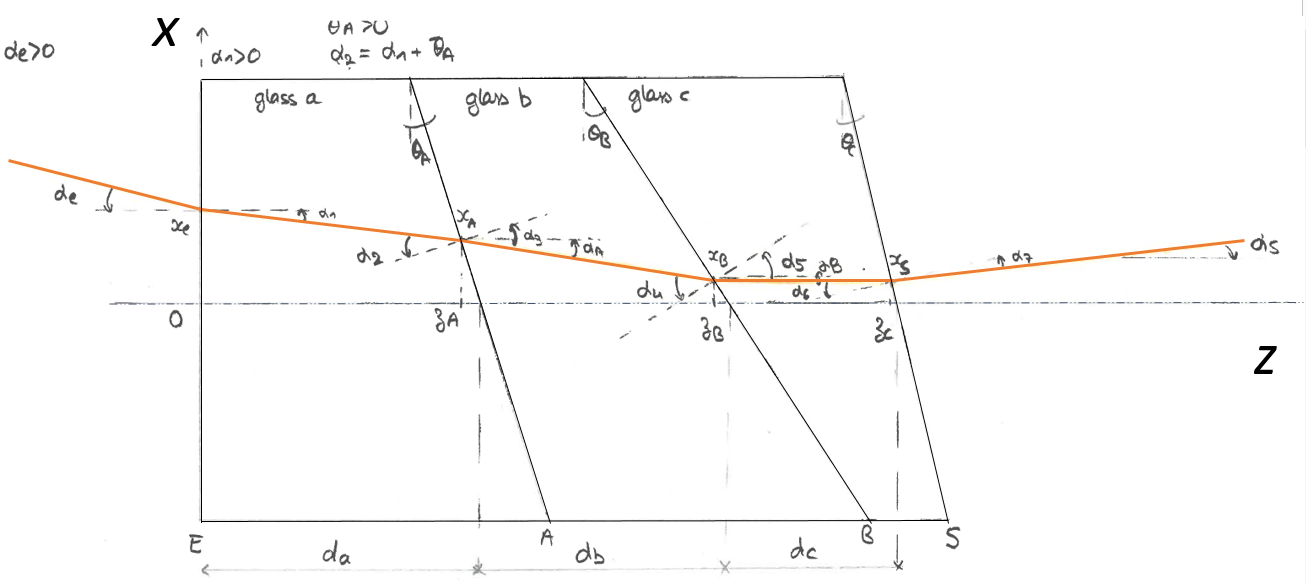
\includegraphics[width = \textwidth]{images/ADCgeometrie.png}
	\caption{Sketch of the refraction through the ADC}\label{fig:ADCgeometrie}
	\centering
\end{figure}
The refractive index of the I-th glass is $n_I(\lambda_i)$. To simplify the notation, we just write $n_I$.
We apply the sign convention described in the course material~\cite{coursOptLJT}.
\paragraph*{At the entrance we have the vector}
$\begin{bmatrix}x_E \\ z_E = 0 \\ n_0\sin\alpha_E\end{bmatrix}$
 
\paragraph*{At the entrance 0E, we have a refraction}
$\begin{bmatrix}x_E \\ z_E = 0 \\ n_A\sin\alpha_1\end{bmatrix}$\\

which gives :\\

$\alpha_1 = \arcsin\left(\frac{n_0}{n_A}\sin\alpha_E\right) $

\paragraph*{At the first interface AB, we arrive with the coordinates}

$\begin{bmatrix}x_A \\ z_A \\ n_A\sin\left(\alpha_2\right)\end{bmatrix}$
\begin{figure}[H]
\centering
	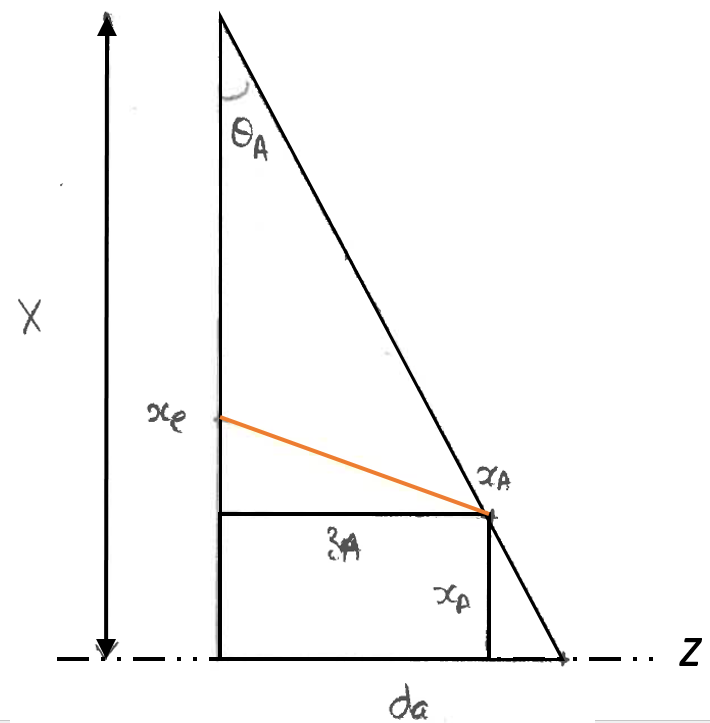
\includegraphics[width = .3\textwidth]{images/triangleGeo.png}
	\caption{Decomposition of the parameters at an interface}\label{fig:triangle}
	\centering
\end{figure}
We can determine this vector using the following equations from figure~\ref{fig:triangle} :\\

$X = \frac{d_A}{\tan\theta_A}$ ; $\frac{X-x_A}{X} = \frac{z_A}{d_A}$ ; $z_A = \frac{x_E-x_A}{\tan\alpha_1}$\\

Then we find :\\
$\left \{
   \begin{array}{r c l}
      x_A  & = & \frac{x_E-d_A\tan\alpha_1}{1-\tan\alpha_1\tan\theta_A} \\
      z_A   & = & \frac{x_E-x_A}{\tan\alpha1} \\
      \alpha_2 & = & \alpha_1+\theta_A
   \end{array}
\right.$

\paragraph*{At the interface AB, we have a refraction}
$\begin{bmatrix}x_A \\ z_A \\ n_B\sin\alpha_3\end{bmatrix}$\\

which gives :\\

$\alpha_3 = \arcsin\left(\frac{n_A}{n_B}\sin\alpha_2\right) $

\paragraph*{At the interface BC, we arrive with the coordinates}

$\begin{bmatrix}x_B \\ z_B \\ n_B\sin\left(\alpha_4\right)\end{bmatrix}$\\

We can determine this vector using the following equations from figure~\ref{fig:triangle} :\\

$X = \frac{x_A}{\tan\alpha_A}$ ; $\frac{x_B}{X-Q-d_B+m} = \tan\alpha_A$ ; $m = d_A+d_B-z_B$ ; $m = x_B\tan\theta_B$ ; $Q = d_A-z_A$ ; $\alpha_A = \alpha_3+\theta_A$\\

Then we find :\\
$\left \{
   \begin{array}{r c l}
      x_B  & = & \frac{x_A-\tan\alpha_A\left(d_A+d_B-z_A\right)}{1-\tan\alpha_A\tan\theta_B} \\
      z_B   & = & d_A+d_B-x_B\tan\theta_B \\
      \alpha_4 & = & \alpha_A+\theta_B
   \end{array}
\right.$

\paragraph*{At the interface BC, we have a refraction}
$\begin{bmatrix}x_B \\ z_B \\ n_C\sin\alpha_5\end{bmatrix}$\\

which gives :\\

$\alpha_5 = \arcsin\left(\frac{n_B}{n_C}\sin\alpha_4\right) $


\paragraph*{At the interface C0, we arrive with the coordinates}

$\begin{bmatrix}x_C \\ z_C \\ n_C\sin\left(\alpha_6\right)\end{bmatrix}$\\

We can determine this vector using the following equations from figure~\ref{fig:triangle} :\\

$X = \frac{x_B}{\tan\alpha_B}$ ; $\frac{x_C}{X-Q-d_C+m} = \tan\alpha_B$ ; $m = d_A+d_B-z_B$ ; $m = x_C\tan\theta_C$ ; $Q = d_A+d_B-z_B$ ; $\alpha_B = \alpha_5+\theta_B$\\

Then we find :\\
$\left \{
   \begin{array}{r c l}
      x_C  & = & \frac{x_B-\tan\alpha_B\left(d_A+d_B+d_C-z_B\right)}{1-\tan\alpha_B\tan\theta_C} \\
      z_B   & = & d_A+d_B+d_C-x_C\tan\theta_C \\
      \alpha_6 & = & \alpha_B+\theta_C
   \end{array}
\right.$

\paragraph*{At the interface C0, we have a refraction}
$\begin{bmatrix}x_C \\ z_C \\ n_0\sin\alpha_7\end{bmatrix}$\\

which gives :\\

$\alpha_7 = \arcsin\left(\frac{n_C}{n_0}\sin\alpha_6\right) $\\

\paragraph*{The output angle with respect to the optical axis}\
$\alpha_S = \alpha_7-\theta_C$
This $\alpha_S$ is the dispersion angle of the prism : $R_{prism} = \alpha_S$.





\subsubsection{The metric definition}
Now we have computed the dispersion of the atmosphere and the ADC. We want the smallest total dispersion so we investigate all ADC configurations in order to minimize it. The metric we use comes from~\cite{Tendulkar} to calculate the efficiency of our prism combination :
\begin{equation}
	\text{Eff}\left(\text{prism parameters}\right) = \sum_{\lambda_i}\left(R_{prism}\left(\lambda_i;\text{prism parameters}\right) - R_{atm}\left(\lambda_i\right)\right)^2
\end{equation}


\subsubsection{Internal reflection}
In parallel of the dispersion computation, we calculate the total internal reflection of the ADC. If the refractive index of two joint glasses are too different then we will loose a lot of intensity reflected on the interface. The external faces of the ADC will be coated. The determination of the total internal reflectivity is developed below.\\
The parameters are :
\begin{itemize}
	\item $\alpha_Z = [\alpha_E;\alpha_1;\alpha_A;\alpha_B;\alpha_S]$ [rad] array of the rays angle wrt the optical axis
	\item $\alpha_I = [\alpha_1;\alpha_2;\alpha_3;\alpha_4;\alpha_5;\alpha_6;\alpha_7]$ [rad] array of the rays angles wrt the normal the vertex (refraction angle)
	\item $n = [n_0;n_A;n_B;n_C;n_0]$ medium refractive index
	\item $d = [z_A,z_B-z_A,z_C-z_B]$ [mm] distances on the optical axis between each medium change on the ray path
\end{itemize}

At the 1rst interface AB, we have :
\begin{equation}
	r[1] = \frac{n[3]\cos\alpha_I[2]-n[2]\cos\alpha_I[3]}{n[3]\cos\alpha_I[2]+n[2]\cos\alpha_I[3]}
\end{equation}
Taking the recursive initialization term $U(1) = r(1)$ we have for p = 2:\\
\begin{eqnarray}
	r[p] &= &\frac{n[p+1]\cos\left(\alpha_I[p]\right)-n[p]\cos\left(\alpha_I[p+1]\right)}{n[p+1]\cos\left(\alpha_I[p]\right)+n[p]\cos\left(\alpha_I[p+1]\right)}\\
	U[p] &= &\frac{U[p-1]+r[p]\exp\left(\frac{2\pi}{\lambda}\cos\left(\alpha_Z[p]\right)\,d[p-1]\right)}{1+U[p-1]\,r[p]\exp\left(\frac{2\pi}{\lambda}\cos\left(\alpha_Z[p]\right)\,d[p-1]\right)}\label{eq:Up}
\end{eqnarray}
Using equation~\eqref{eq:Up} we can calculate the reflection coefficient for $(p+1)$ number of glasses. In our case we have only 3 glasses so the total reflection (without taking external faces into account) is $U[2]$.

\subsection{ADC design optimization}
The efficiency of a combination (glass, angle, thickness) is computed by the function \textit{Refraction\_calculs\_geometriques\_20180302.m}. The \textit{fmincon} Matlab algorithm is used to find minimum of this constrained nonlinear multivariable function. The parameters are the geometrical coefficients for one set of glass. When the optimum is found for a combination of glass, the efficiency and internal reflection are given as outputs.\\

The global matrix is made from two for-loops that look for all glasses from the catalogues Schott and Ohara. We decide to have the same glass type for the external wedges in order to simplify the anti-reflection coating process. This would give us the possibility to coat the prism at once and so reduce the cost. The refractive index of the middle wedge glass is chosen larger than the middle one to save effort and cost on the coating. In the optimization process on Matlab, when this refractive index (for $\lambda_\text{mean}$ is larger than external one the loop stops. The outputs are set to 20'000 (arbitrarily large to oust them).\\
The wavelength for which the refraction is calculated are taken from the Nuvu camera quantum efficiency curve~: $\lambda_\text{min}~=~300$ nm, $\lambda_\text{mean}~=~600$ nm and $\lambda_\text{max}~=~1000$ nm. The zenith angle is set to 70\degree.



\section{DimensionnementOAPs.py}\label{app:DimensionnementOAPs}
\lstinputlisting[language=Python]{../DimensionnementOAPs.py}





















\end{document}